\documentclass{l4dc2027}
% Numbers come from results3.tex, written by tfl/make_results3.py from the run files.
\title[Learning constrained regions of attraction]{Learning Constrained Regions of Attraction: Transverse Feedback
Linearization and Beyond}
\usepackage{times}
\usepackage{booktabs}
\usepackage{multirow}
\usepackage{float}
\usepackage{xcolor}
% written by make_results3.py from the run files; do not edit
\newcommand{\TBD}[1]{\textcolor{red}{[#1]}}
\newcommand{\resAbsCirc}{75.8\,\%}
\newcommand{\resAbsInnerCirc}{6.4\,\%}
\newcommand{\resRoaCirc}{84.8\,\%}
\newcommand{\resCovCircMean}{74.0\,\%}
\newcommand{\resCeilCirc}{84.8\,\%}
\newcommand{\resCeilFracCirc}{87\,\%}
\newcommand{\resQuadCirc}{8.3\,\%}
\newcommand{\resPinnTFLCirc}{6.4\,\%}
\newcommand{\resDzTFLCirc}{11.3\,\%}
\newcommand{\resSafetyCirc}{33.5\,\%}
\newcommand{\resGapCirc}{37.1}
\newcommand{\resWholeLevelMaxCirc}{0.9947}
\newcommand{\resPinnBothMaxCirc}{11.3\,\%}
\newcommand{\resZubovMaxCirc}{11.3\,\%}
\newcommand{\resOtherMaxCirc}{36.9\,\%}
\newcommand{\resWholeCirc}{36.9\,\%}
\newcommand{\resWholeUnionCirc}{54.1\,\%}
\newcommand{\resPinnCirc}{9.4\,\%}
\newcommand{\resRawCircMean}{69.5\,\%}
\newcommand{\resRepairGainCirc}{+4.5}
\newcommand{\resRichMaxCirc}{18.2\,\%}
\newcommand{\resKeptCirc}{zero}
\newcommand{\resCeilNineCirc}{73.0\,\%}
\newcommand{\resCtwoMinCirc}{0.98}
\newcommand{\resCtwoMaxCirc}{0.99}
\newcommand{\resSeedZeroCirc}{69.8\,\%}
\newcommand{\resAbsSin}{75.0\,\%}
\newcommand{\resAbsInnerSin}{1.1\,\%}
\newcommand{\resRoaSin}{95.0\,\%}
\newcommand{\resCovSinMean}{70.4\,\%}
\newcommand{\resCeilSin}{76.6\,\%}
\newcommand{\resCeilFracSin}{92\,\%}
\newcommand{\resQuadSin}{2.1\,\%}
\newcommand{\resPinnTFLSin}{4.0\,\%}
\newcommand{\resDzTFLSin}{1.1\,\%}
\newcommand{\resSafetySin}{29.5\,\%}
\newcommand{\resGapSin}{12.8}
\newcommand{\resWholeLevelMaxSin}{0.9855}
\newcommand{\resPinnBothMaxSin}{4.0\,\%}
\newcommand{\resZubovMaxSin}{4.0\,\%}
\newcommand{\resOtherMaxSin}{57.6\,\%}
\newcommand{\resWholeSin}{57.6\,\%}
\newcommand{\resWholeUnionSin}{62.8\,\%}
\newcommand{\resRawSinMean}{58.0\,\%}
\newcommand{\resRepairGainSin}{+12.4}
\newcommand{\resRichMaxSin}{2.5\,\%}
\newcommand{\resKeptSin}{zero}
\newcommand{\resCeilNineSin}{57.4\,\%}
\newcommand{\resCtwoMinSin}{0.96}
\newcommand{\resCtwoMaxSin}{0.98}
\newcommand{\resSeedZeroSin}{57.2\,\%}
\newcommand{\resAbsQuad}{12.8\,\%}
\newcommand{\resAbsInnerQuad}{0.0\,\%}
\newcommand{\resRoaQuad}{56.2\,\%}
\newcommand{\resCovQuadMean}{9.2\,\%}
\newcommand{\resCeilQuad}{33.3\,\%}
\newcommand{\resCeilFracQuad}{28\,\%}
\newcommand{\resQuadQuad}{0.0\,\%}
\newcommand{\resPinnTFLQuad}{0.0\,\%}
\newcommand{\resDzTFLQuad}{0.0\,\%}
\newcommand{\resSafetyQuad}{8.4\,\%}
\newcommand{\resGapQuad}{9.1}
\newcommand{\resWholeLevelMaxQuad}{0.0007}
\newcommand{\resPinnBothMaxQuad}{0.0\,\%}
\newcommand{\resZubovMaxQuad}{0.0\,\%}
\newcommand{\resOtherMaxQuad}{0.1\,\%}
\newcommand{\resWholeQuad}{0.1\,\%}
\newcommand{\resWholeUnionQuad}{0.3\,\%}
\newcommand{\resRawQuadMean}{9.4\,\%}
\newcommand{\resRepairGainQuad}{-0.2}
\newcommand{\resRichMaxQuad}{0.0\,\%}
\newcommand{\resKeptQuad}{four}
\newcommand{\resDrawMaxQuad}{2.2}
\newcommand{\resCeilNineQuad}{79.8\,\%}
\newcommand{\resCtwoMinQuad}{0.28}
\newcommand{\resCtwoMaxQuad}{0.45}
\newcommand{\resSeedZeroQuad}{9.4\,\%}
\newcommand{\resUnsafeKCirc}{1}
\newcommand{\resUnsafeInCirc}{644\,243}
\newcommand{\resUnsafeEpsCirc}{$1.7\times10^{-5}$}
\newcommand{\resUnsafeTimeCirc}{5}
\newcommand{\resUnsafeKSin}{0}
\newcommand{\resUnsafeInSin}{713\,563}
\newcommand{\resUnsafeEpsSin}{$1.4\times10^{-5}$}
\newcommand{\resUnsafeTimeSin}{5}
\newcommand{\resUnsafeKQuad}{2}
\newcommand{\resUnsafeInQuad}{72\,523}
\newcommand{\resUnsafeEpsQuad}{$1.9\times10^{-5}$}
\newcommand{\resUnsafeTimeQuad}{8}
\newcommand{\resUnsafeDis}{41}
\newcommand{\resUnsafeAgree}{38}
\newcommand{\resUnsafeCmp}{9000}
\newcommand{\resUnsafeCons}{3}
\newcommand{\resUnsafeDisInS}{none}
\newcommand{\resUnsafeTotal}{3}
\newcommand{\resUnsafeConfirmed}{3}
\newcommand{\resUnsafeEpsMax}{$1.9\times10^{-5}$}
\newcommand{\resUnsafeTimeMax}{8}
\newcommand{\resContactCirc}{0.1252}
\newcommand{\resCICirc}{0.1050}
\newcommand{\resFloorCirc}{0.7\,\%}
\newcommand{\resContactSin}{0.0563}
\newcommand{\resCISin}{0.0509}
\newcommand{\resFloorSin}{5.0\,\%}
\newcommand{\resContactQuad}{0.0056}
\newcommand{\resCIQuad}{0.0006}
\newcommand{\resFloorQuad}{57.9\,\%}
\newcommand{\resRefNoiseMax}{0.74\,\%}
\newcommand{\resRefNoiseCirc}{0.24\,\%}
\newcommand{\resRefNoiseSin}{0.24\,\%}
\newcommand{\resRefNoiseQuad}{0.74\,\%}
\newcommand{\resProbeKeepCirc}{70.3\,\%}
\newcommand{\resProbeAltCirc}{66.6\,\%}
\newcommand{\resProbeKeepSin}{57.2\,\%}
\newcommand{\resProbeAltSin}{42.4\,\%}
\newcommand{\resProbeOrigQuad}{0.2\,\%}
\newcommand{\resProbeBestQuad}{13.4\,\%}
\newcommand{\resProbeWideQuad}{13.7\,\%}
\newcommand{\resProbeQuadN}{eight}
\newcommand{\resCollapseExtra}{one}
\newcommand{\resOracleMaxCirc}{20.2\,\%}
\newcommand{\resOracleMaxSin}{33.7\,\%}
\newcommand{\resOracleMaxQuad}{2.4\,\%}
\newcommand{\resFPMax}{0.000\,\%}
\newcommand{\resFPSentence}{No reference state lies}
\newcommand{\resIidFailures}{six}
\newcommand{\resRepairGain}{5.6}
\newcommand{\resRepairKept}{4}
\newcommand{\resTimeTrain}{15 to 27 minutes}
\newcommand{\resTimeCert}{1 to 5 minutes}
\newcommand{\resTimeRepair}{1 to 16 minutes}
\newcommand{\resTimeInner}{110 to 3626 seconds per case}
\newcommand{\resPinnVdpOne}{98.9\,\%}
\newcommand{\resDzVdpOne}{97.2\,\%}
\newcommand{\resSeedVdpOne}{98.6\,\%}
\newcommand{\resPinnBestVdpOne}{99.4\,\%}
\newcommand{\resPinnWorstVdpOne}{98.5\,\%}
\newcommand{\resSosVdpOne}{99.1\,\%}
\newcommand{\resPinnVdpThree}{91.5\,\%}
\newcommand{\resDzVdpThree}{94.8\,\%}
\newcommand{\resSeedVdpThree}{90.4\,\%}
\newcommand{\resPinnBestVdpThree}{95.4\,\%}
\newcommand{\resPinnWorstVdpThree}{88.0\,\%}
\newcommand{\resSosVdpThree}{93.3\,\%}
\newcommand{\resPinnPend}{99.2\,\%}
\newcommand{\resDzPend}{91.5\,\%}
\newcommand{\resSeedPend}{91.6\,\%}
\newcommand{\resPinnBestPend}{99.4\,\%}
\newcommand{\resPinnWorstPend}{99.0\,\%}
\newcommand{\resSosPend}{53.8\,\%}
\newcommand{\resPinnConThree}{61.2\,\%}
\newcommand{\resDzConThree}{70.9\,\%}
\newcommand{\resSeedConThree}{82.8\,\%}
\newcommand{\resPinnBestConThree}{65.5\,\%}
\newcommand{\resPinnWorstConThree}{57.4\,\%}
\newcommand{\resSosConThree}{10.0\,\%}
\newcommand{\resPinnPower}{98.6\,\%}
\newcommand{\resDzPower}{90.6\,\%}
\newcommand{\resSeedPower}{92.5\,\%}
\newcommand{\resPinnBestPower}{99.3\,\%}
\newcommand{\resPinnWorstPower}{98.4\,\%}
\newcommand{\resSosPower}{43.8\,\%}
\newcommand{\resSeedObsVdpOne}{85.5\,\%}
\newcommand{\resDzObsVdpOne}{87.4\,\%}
\newcommand{\resPinnObsVdpOne}{80.9\,\%}
\newcommand{\resUnionObsVdpOne}{89.9\,\%}
\newcommand{\resSeedObsVdpTwo}{66.5\,\%}
\newcommand{\resDzObsVdpTwo}{78.6\,\%}
\newcommand{\resPinnObsVdpTwo}{56.1\,\%}
\newcommand{\resUnionObsVdpTwo}{73.4\,\%}
\newcommand{\resSeedObsPowTwo}{74.0\,\%}
\newcommand{\resDzObsPowTwo}{86.4\,\%}
\newcommand{\resPinnObsPowTwo}{73.1\,\%}
\newcommand{\resUnionObsPowTwo}{81.0\,\%}
\newcommand{\resSeedObsPowFour}{64.8\,\%}
\newcommand{\resDzObsPowFour}{90.8\,\%}
\newcommand{\resPinnObsPowFour}{76.0\,\%}
\newcommand{\resUnionObsPowFour}{75.7\,\%}
\newcommand{\resObsNoObsMin}{5.3\,\%}
\newcommand{\resObsNoObsMax}{46.4\,\%}
\newcommand{\resSosLiuSetVdpOne}{78.7\,\%}
\newcommand{\resSosLiuSetVdpThree}{48.2\,\%}
\newcommand{\resSosStudyOurs}{93.4\,\%}
\newcommand{\resSosStudyShape}{56.2\,\%}
\newcommand{\resSosStudyInitx}{73.1\,\%}
\newcommand{\resSosStudySone}{57.1\,\%}
\newcommand{\resSosStudyBoxGap}{1.3}
\newcommand{\resSosStudyNobox}{94.7\,\%}
\newcommand{\resSosLevelConThree}{0.999}
\newcommand{\resSosTimePend}{14}
\newcommand{\resSosTimePower}{3}
\newcommand{\resBenchFPSentence}{No reference state lies}
\newcommand{\resPinnVdpOneMean}{85.3\,\%}
\newcommand{\resPinnVdpThreeLow}{78.2\,\%}
\newcommand{\resPinnVdpThreeMin}{84.0}
\newcommand{\resPinnVdpThreeMax}{86.6\,\%}
\newcommand{\resBenchFPMax}{0.000\,\%}
\newcommand{\resSosGapMax}{0.6}
\newcommand{\resBenchMin}{73.4\,\%}
\newcommand{\resBenchMax}{99.2\,\%}
\newcommand{\resBenchSeedMin}{82.8\,\%}
\newcommand{\resBenchSeedMax}{98.6\,\%}
\newcommand{\resCoreRoaMin}{2.0\,\%}
\newcommand{\resCoreRoaMax}{43.7\,\%}
\newcommand{\resCoreTimeMax}{12}
\newcommand{\resRedN}{39}
\newcommand{\resSeedsN}{60}
\newcommand{\resRecN}{37}
\newcommand{\resRecLo}{57.4}
\newcommand{\resRecHi}{99.4}
\newcommand{\resRestN}{two}
\newcommand{\resGridLowerMax}{0.007}
\newcommand{\resPinnWinsN}{eight}
\newcommand{\resAllUnsafeMax}{four}
\newcommand{\resOUnsafeList}{2, 0, 0 and 2}
\newcommand{\resOUnsafeEpsMax}{$1.9\times10^{-5}$}
\newcommand{\resOUnsafeDis}{0}
\newcommand{\resBUnsafeList}{3, 3, 4, 1 and 0}
\newcommand{\resBUnsafeEpsMax}{$2.3\times10^{-5}$}
\newcommand{\resBUnsafeTimeMax}{24}
\newcommand{\resBUnsafeCmp}{30\,000}
\newcommand{\resBUnsafeDis}{0}
\newcommand{\resBUnsafeTotal}{11}
\newcommand{\resBUnsafePend}{four}
\newcommand{\resBUnsafePendSeeds}{one}
\newcommand{\resBUnsafeDisWord}{in no case}
\newcommand{\resBUnsafeConfirmed}{15}

\newcommand{\Oad}{\Omega_{\mathrm{ad}}}
\newcommand{\R}{\mathbb{R}}
\newcommand{\D}{\mathcal D}
\newcommand{\I}{\mathcal I}
\newcommand{\Tm}{\mathcal T}
\newcommand{\qex}{q_{\mathrm{ex}}}
\newcommand{\dist}{\operatorname{dist}}
\newcommand{\relu}{\operatorname{relu}}
\newtheorem{problem}{Problem}
\newtheorem{assumption}{Assumption}

\coltauthor{%
 \Name{Abdullah Waqar Malik} \Email{amalik.bscs22seecs@seecs.edu.pk}\\
 \addr School of Electrical Engineering and Computer Science, National University of Sciences and Technology,
 Islamabad, Pakistan
 \AND
 \Name{Hamza Tariq} \Email{ht299@njit.edu}\\
 \addr New Jersey Institute of Technology, Newark, NJ, USA
 \AND
 \Name{Adeel Akhtar} \Email{adeel.akhtar@njit.edu}\\
 \addr New Jersey Institute of Technology, Newark, NJ, USA%
}

\begin{document}

\maketitle

\vspace{-0.3in}

\begin{abstract}%
\looseness -1 Transverse feedback linearization (TFL) makes a vehicle follow a path, but the controller is undefined on a singular set,
such as zero speed for a unicycle or zero thrust for a quadrotor. Because of this set and the state limits, only some
initial states converge to the path. This constrained region of attraction is unknown, yet it tells us where the controller
can be safely switched on. Wherever the controller is defined and the limits hold, the transverse dynamics are exactly linear, so the state-constrained Zubov
value function splits into a known quadratic cost-to-go and a safety value function. We learn only the safety value
function, without infinite-horizon labels, with a network whose sublevel sets respect the constraints by construction. Our
estimate has an inner layer verified by interval branch and bound and an outer layer tested on samples. On a unicycle following a
circle and a sinusoid and on a planar quadrotor, the estimate covers on average \resCovCircMean, \resCovSinMean\ and
\resCovQuadMean\ of the simulated region of attraction. The quadratic cost-to-go alone and two physics-informed neural
network (PINN) solvers of Zubov's equation, the Zubov PINN and the Dirichlet-Zubov PINN, cover on average at most \resZubovMaxCirc, \resZubovMaxSin\ and
\resZubovMaxQuad. With a quadratic form from the linearization, the same learning applies to general closed loops. On nine equilibrium
benchmarks the estimate is comparable to the PINN and sum-of-squares baselines and covers the most on \resObsBestCount\ of the five with obstacles.%
\end{abstract}

\begin{keywords}%
Region of attraction, transverse feedback linearization, Zubov equation, state constraints, value iteration%
\end{keywords}

% ======================================================================================================
\section{Introduction}\label{sec:intro}

\looseness -1 Transverse feedback linearization (TFL) solves path following as a set-stabilization problem. A change of coordinates and a
feedback that inverts a decoupling matrix make the dynamics transverse to the path linear and exponentially stable, while
the tangential dynamics move the vehicle along it \citep{nielsen2006,nielsen2008}. The construction has been worked out for
car-like robots \citep{akhtar2011,akhtar2015} and quadrotors \citep{akhtar2012,allawati2026}. Its guarantee is local. The
decoupling matrix loses rank on a singular set, at zero speed for the dynamically extended unicycle and at zero thrust for a
quadrotor, and the vehicle must respect state limits. A trajectory that starts far from the path can reach the singular set
even though its transverse error would have decayed. The stability theorem says that the path attracts a neighbourhood, and
it does not say how large this neighbourhood is. We ask which initial states of a given TFL controller converge to the path
while the closed loop stays well defined and inside its state limits.

These states form the constrained region of attraction. It is the set on which a Zubov value function with an obstacle term
is finite \citep{gruene2015}, an extension of Zubov's equation \citep{camilli2001} to state constraints. Grid solvers for this
equation stop at low dimension, and sum-of-squares methods need polynomial dynamics \citep{xue2020}. Neural solvers of Zubov equations learn the value function of an equilibrium or, in discrete
time, of a compact invariant set, using simulated labels \citep{liu2025,kang2023,mengliu2026,serry2025,serry2026} or a
short-time operator \citep{meng2024}. Those that certify the result use formal verifiers, on systems of two to four dimensions
unless the system is compositional. Reachability computations on grids have produced feedback-linearizing controllers together with the set of states on which they are valid
\citep{oishi2006}. Path-following model predictive control uses sublevel sets of a transverse quadratic form as terminal
regions \citep{faulwasser2016}. We found no estimate of the constrained region of attraction of a TFL controller under a singular
decoupling matrix, and no method that learns one (Appendix~\ref{app:related}).

\looseness -1 Our approach uses the structure of the closed loop. We define an admissible set constituting states where the controller is defined and the state limits hold. The transverse dynamics are exactly linear on this set, so a trajectory that never leaves it converges
to the path. Convergence therefore reduces to forward invariance, and the running-cost part of the Zubov value function is known
in closed form. Only the remaining part, which encodes the constraints, has to be learned. Our contributions are the following.
\begin{itemize}
\item We show that the constrained region of attraction of a TFL controller is the largest forward invariant subset of its
admissible set, and that its Zubov value function is the sum of a known quadratic cost-to-go and a safety value function.
\item We learn only the safety value function, with a network whose finite sublevel sets avoid the singular set and the state
limits by construction, and without infinite-horizon labels. With a quadratic form from the linearization, the same learning
applies to general closed loops.
\item We give a two-layer estimate of the constrained region of attraction: an inner layer verified by interval branch and bound, and an outer
layer tested on samples, with confidence bounds on the missed counterexamples and on the states it wrongly includes.
\end{itemize}
\looseness -1 Simulations on a unicycle, a planar quadrotor and nine equilibrium benchmarks compare these estimates with the quadratic baseline,
sum-of-squares, the Zubov PINN and the Dirichlet-Zubov PINN.

\paragraph{Notation.} For a function $\varphi$ and a vector field $f$, $L_f\varphi=\nabla\varphi\cdot f$ is the Lie derivative.
We write $y(t;x)$ for the solution of the closed loop from $x$ in physical time, $\dist(x,M)=\inf_{m\in M}\|x-m\|$,
$\relu(t)=\max\{t,0\}$, $B^\circ$ for the interior of a box $B$, and $\{v<c\}$ for a sublevel set.

% ======================================================================================================

\vspace{-0.15in}

\section{Preliminaries and Problem Formulation}\label{sec:problem}

\subsection{Transverse feedback linearization and the admissible set}\label{sec:tfl}
Consider a control-affine system $\dot x=f(x)+g_1(x)u_1+g_2(x)u_2$ with state $x\in\R^n$ and position output
$p(x)\in\R^2$. A planar path is the zero set of a smooth function $\alpha$ of the position, and a smooth function $\varpi$
of the position measures progress along it. Both outputs are assumed to have the same relative degree $r$, so that
$L_{g_j}L_f^k\alpha=L_{g_j}L_f^k\varpi=0$ for $k<r-1$. The transverse coordinates are
$\xi=(\alpha,L_f\alpha,\dots,L_f^{r-1}\alpha)$, the tangential coordinates are $\eta=(\varpi,L_f\varpi,\dots,L_f^{r-1}\varpi)$,
and $\Tm(x)=(\eta,\xi)$ is the change of coordinates. The decoupling matrix $D(x)$ has rows
$(L_{g_1}L_f^{r-1}\varpi,L_{g_2}L_f^{r-1}\varpi)$ and $(L_{g_1}L_f^{r-1}\alpha,L_{g_2}L_f^{r-1}\alpha)$. The TFL controller is
\begin{equation}\label{eq:tfl}
u=D(x)^{-1}\Big(-\begin{bmatrix}L_f^{r}\varpi\\ L_f^{r}\alpha\end{bmatrix}+\begin{bmatrix}\nu_\parallel\\ \nu_\perp\end{bmatrix}\Big),
\qquad \nu_\perp=k^\top\xi,\qquad \nu_\parallel=k_\eta^\top(\eta_2-\bar\eta,\eta_3,\dots,\eta_r),
\end{equation}
with gains such that the transverse dynamics $\dot\xi=A_\xi\xi$ and the dynamics of the tangential speed $\eta_2=L_f\varpi$ are
exponentially stable, and with $\bar\eta$ the reference tangential speed. The error coordinates
$z(x)=(\xi,\eta_2-\bar\eta,\eta_3,\dots,\eta_r)$ vanish when the vehicle follows the path at the reference tangential speed. Wherever $D(x)$
is invertible and $\Tm$ is a local diffeomorphism, the closed loop satisfies $\dot z=Az$ exactly, with $A$ Hurwitz and block diagonal.

The controller is undefined where $\det D(x)=0$. The coordinates fail to be a chart where the Jacobian $J_\Tm$ of $\Tm$ is singular, and the function
$\varpi$ is undefined at the centre of a circular path, where its gradient is unbounded. We call the union of these sets the
singular set. With thresholds $\epsilon_D,\epsilon_\Tm,\epsilon_\varpi>0$ and a box $B$ of state limits, the admissible set is
\begin{equation}\label{eq:oad}
\Oad=\{x:\ |\det D(x)|>\epsilon_D,\ |\det J_\Tm(x)|>\epsilon_\Tm,\ \|\nabla\varpi(x)\|^{-1}>\epsilon_\varpi\}\cap B^\circ,
\end{equation}
an open set on which the closed-loop field $f_{\mathrm{cl}}$ is smooth. We call the three inequalities in \eqref{eq:oad} the
regularity constraints. The field grows large near the singular set because $u\sim1/\det D$, which makes a fixed integration step
inaccurate. We therefore integrate the normalized field $\bar f=f_{\mathrm{cl}}/a$, with $a=\sqrt{1+\|Sf_{\mathrm{cl}}\|^2}$ and $S$
the diagonal matrix of inverse half-widths of $B$. This change of time scale preserves orbits and the sets defined below. All
numerical step lengths in the training and the tests are measured in the time of $\bar f$, which we call normalized time.

\paragraph{The two systems.} The unicycle has state $(x_1,x_2,x_3,x_4)$ (position, heading, speed $1+x_4$), inputs
acceleration and turn rate, $r=2$, and $\det D=\pm(1+x_4)\det[\nabla\varpi;\nabla\alpha]$, which vanishes at zero speed. The paths
are the unit circle with $\varpi=\operatorname{atan2}(x_2,x_1)$ and the sinusoid $x_2=\sin x_1$ with $\varpi=x_1$. The
planar quadrotor has state $(p_1,p_2,w_1,w_2,\vartheta,T)$ (position, velocity, tilt, thrust), with the thrust rate and the
tilt rate as inputs and $r=3$. For the unit circle in the vertical plane $\det D=-2T$, so its controller is singular at
zero thrust. Appendix~\ref{app:systems} gives the equations, gains, thresholds and boxes.

\subsection{Target set and constrained region of attraction}
The target set is $M=\{x\in\overline{\Oad}:\ z(x)=0\}$, the path traversed at the reference tangential speed. Our results rest on
the following assumption.

\begin{assumption}\label{ass:main}
(a) The closed-loop field $f_{\mathrm{cl}}$ is smooth on a neighbourhood of $\overline{\Oad}$.
(b) On $\Oad$ the error coordinates satisfy $\dot z=Az$ with $A$ Hurwitz.
(c) The target set satisfies $M\subset\Oad$.
\end{assumption}

\looseness -1 Assumption~\ref{ass:main} is mild. On $\overline{\Oad}$ the
regularity constraints hold with $\ge$, so positive thresholds keep $\overline{\Oad}$ and a neighbourhood of it off the singular set, which gives
part (a). Part (b) is the property of TFL stated in Section~\ref{sec:tfl}, and it only requires stabilizing gains. Part (c) asks that the path,
traversed at the reference tangential speed, lie inside the state limits and off the singular set. It holds whenever the box and the reference tangential speed leave a
margin around the path, and Appendix~\ref{app:systems} checks it in each case. Under Assumption~\ref{ass:main}, the set $M$ is compact, and it
is forward invariant because $\dot z=Az$ on $\Oad$. The constrained region of attraction of $M$ is
\begin{equation}\label{eq:D}
\D(M)=\bigl\{x\in\Oad:\ y(t;x)\in\Oad\ \text{for all } t\ge0\ \text{ and }\ \dist(y(t;x),M)\to0\bigr\}.
\end{equation}
A trajectory from a state outside $\D(M)$ leaves $\Oad$, by violating a regularity constraint or a state limit, or does not converge. Deciding membership in
$\D(M)$ directly requires simulating each initial state.

\begin{problem}\label{prob:main}
Given the closed loop \eqref{eq:tfl} on $\Oad$, compute a set $\Omega\subset\D(M)$ that contains a neighbourhood of
$M$, is described by sublevel sets of explicit functions, is obtained without simulating trajectories until they
converge, and covers as large a share of $\D(M)$ as possible.
\end{problem}

% ======================================================================================================

\vspace{-0.2in}

\section{Methodology}\label{sec:method}

We address Problem~\ref{prob:main} with a two-layer estimate $\Omega=\I\cup\{v<c_2\}$. The inner layer $\I$ is a sublevel set
of a known quadratic form, and its inclusion in $\D(M)$ is verified by interval arithmetic. The outer layer $\{v<c_2\}$ is a sublevel set of a learned
function $v$, and its inclusion is tested on samples. Section~\ref{sec:guarantees} states the status of each part.

\subsection{Decomposition of the value function}
Let $\zeta=S_zz$ be the error coordinates scaled by the median of $|z|$ over admissible samples, let $Q\succ0$, and
let $P$ solve $\tilde A^\top P+P\tilde A=-Q$ with $\tilde A=S_zAS_z^{-1}$. The quadratic cost-to-go is
$\qex(x)=\zeta(x)^\top P\zeta(x)$. The running cost is $\ell=\gamma\,\zeta^\top Q\zeta$ with a scale $\gamma>0$, and the
obstacle function is
\begin{equation}\label{eq:h}
h(x)=\sum_i\relu\big(b_i/d_i(x)-1\big)^2\ \text{ on }\Oad,\qquad h=\infty\ \text{ off }\Oad,
\end{equation}
where $d_i$ is the signed distance to the $i$-th constraint of \eqref{eq:oad} and $b_i$ a tenth of its median over
admissible samples. The obstacle function is locally Lipschitz, zero on a neighbourhood of $M$ and unbounded at the boundary of
$\Oad$. The state-constrained Zubov value function of \citet{gruene2015} and its bounded transform are
\begin{equation}\label{eq:V}
V(x)=\sup_{t\ge0}\Big[\int_0^t \ell(y(s;x))\,ds+h(y(t;x))\Big],\qquad v(x)=1-e^{-V(x)},
\end{equation}
with $V(x)=\infty$ if the trajectory leaves $\Oad$. Theorem~\ref{thm:gz} in Section~\ref{sec:guarantees} shows that
$\D(M)=\{V<\infty\}=\{v<1\}$.

\begin{lemma}[Decomposition]\label{lem:split}
Let Assumption~\ref{ass:main} hold. On $\Oad$, $L_{f_{\mathrm{cl}}}\qex=-\zeta^\top Q\zeta$. Consequently, along every trajectory in $\Oad$
$\int_0^t\ell(y(s))\,ds=\gamma\qex(x)-\gamma\qex(y(t))$, and
\begin{equation}\label{eq:split}
V(x)=\gamma\qex(x)+\Phi(x),\qquad \Phi(x)=\sup_{t\ge0}\psi(y(t;x)),\qquad \psi=\relu(h-\gamma\qex),
\end{equation}
with $\Phi=\infty$ if the trajectory leaves $\Oad$. In particular $V\ge\gamma\qex$ and $\Phi\ge\psi\ge0$ everywhere, and
for every $\tau>0$ and every $x$ whose trajectory stays in $\Oad$ on $[0,\tau]$,
\begin{equation}\label{eq:dp}
\Phi(x)=\max\Big\{\max_{0\le s\le\tau}\psi(y(s;x)),\ \Phi(y(\tau;x))\Big\}.
\end{equation}
\end{lemma}

The proof is in Appendix~\ref{app:proofs}, and \eqref{eq:dp} is the dynamic programming principle (4.11) of \citet{gruene2015} written for $\Phi$. We call $\psi$ the margin function and $\Phi$ the safety value function, since
\eqref{eq:dp} is the self-consistency equation of an undiscounted safety value function \citep{hsu2021,yu2022}. The lemma has two
consequences for the method. First, only $\Phi$ has to be learned. The function $V$ is finite exactly where $\Phi$ is finite. In
Zubov methods for an equilibrium the integral of the running cost must also be learned, and here it is known on the whole admissible
set. Second, $V$ keeps a known strict decrease. Along a trajectory in $\Oad$, the decrease of Remark~4.3 of \citet{gruene2015} reads $V(y(t))\le V(x)-\gamma\big(\qex(x)-\qex(y(t))\big)$, so
$V$ decreases strictly off $M$ even where $\Phi$ is constant. A safety value function is constant along most trajectories and lacks this
decrease. The bound $V\ge\gamma\qex$ also holds for every function of the form \eqref{eq:split}, and it gives the inclusion of
Theorem~\ref{thm:main}(ii).

When the inner layer is not negligible, we add to $\ell$ an extra running cost $\kappa\rho$ with a constant $\kappa>0$
(Appendix~\ref{app:config}). The function $\rho\in[0,1]$ is a smooth step of $\gamma\qex$ that vanishes below half the level of the inner layer and equals one
above that level, so $\kappa\rho$ steepens $v$ just outside the inner layer. Identity \eqref{eq:dp} then becomes
$\Phi(x)=\max\{\max_{s\le\tau}[C_s+\psi(y(s;x))],\ C_\tau+\Phi(y(\tau;x))\}$, with $C_s$ the integral of $\kappa\rho$ in physical time
along the step.

\subsection{Neural candidate}
We learn $\Phi$ in the form
\begin{equation}\label{eq:ansatz}
\begin{aligned}
\Phi_\theta&=\max\{\psi,\Psi_\theta\},\qquad V_\theta=\gamma\qex+\Phi_\theta,\qquad v_\theta=1-e^{-V_\theta},\\
\Psi_\theta(x)&=\tanh\!\big(\qex(x)/q_0\big)\,\tfrac1\beta\,\mathrm{softplus}\big(\beta\,\mathcal N_\theta(F(x))\big),
\end{aligned}
\end{equation}
and we call $v_\theta$ the candidate. Here $\mathcal N_\theta$ is a multilayer perceptron and $\beta=10$. The features $F(x)$ of $\mathcal N_\theta$ are the normalized state
with angles as sine and cosine, $\tanh(\zeta/3)$, and a bounded logarithm of the distances $d_i$ to the regularity constraints. The constant
$q_0$ is the first percentile of $\qex$ over the collocation points, and the factor $\tanh(\qex/q_0)$ gives $\Psi_\theta=0$ on $M$. The candidate has the structure
of the exact solution. Since $\Phi_\theta\ge\psi$, we have $V_\theta\ge\max\{h,\gamma\qex\}$, and every sublevel set $\{V_\theta<c\}$ with $c<\infty$ lies in
$\{h<c\}\subset\Oad$. The candidate therefore avoids the singular set and the state limits by construction. Where the exact
$\Phi$ equals $\psi$, the candidate reproduces it exactly, and the network only has to raise $\Phi_\theta$ on states whose trajectories
later approach a constraint.

\subsection{Training and level selection}
\paragraph{Fitted value iteration.} Training solves \eqref{eq:dp} by regression. The update comes from the semi-Lagrangian scheme (5.1) of
\citet{gruene2015}, with a frozen target as in reach-avoid reinforcement learning \citep{hsu2021}. \citet{li2025} bootstrap the data term of a Zubov
PINN through the network at the end of a short integration in the same way. Identity \eqref{eq:dp} concerns the orbit only, so it also holds with $\tau$ in normalized time. For every collocation point $x$, we
integrate the normalized field by fourth-order Runge-Kutta over $\tau=0.2$ with eight substeps. We store the end point $x_\tau$, the
running maximum $R_\tau(x)=\max_{s\le\tau}[C_s+\psi(y(s))]$ over the substeps ($\infty$ if a substep leaves $\Oad$) and $C_\tau$. These
quantities do not depend on the network, so they are computed once. With a copy $\bar\theta$ of the averaged weights refreshed after
every epoch, the target is
\begin{equation}\label{eq:target}
\mathcal U(x)=\exp\!\big(-\max\{R_\tau(x),\ C_\tau+\Phi_{\bar\theta}(x_\tau)\}\big)\in[0,1],
\end{equation}
which is bounded even where the exact value is infinite. The loss fits $e^{-\Psi_\theta}$ to the target. Where
$\mathcal U(x)<e^{-\psi(x)}$ the exact $\Phi$ exceeds $\psi$, and the loss term is $(e^{-\Psi_\theta(x)}-\mathcal U(x))^2$. Where
$\mathcal U(x)=e^{-\psi(x)}$ the exact $\Phi$ equals $\psi$, and the loss term is $\relu(\mathcal U(x)-e^{-\Psi_\theta(x)})^2$, which only asks
$\Psi_\theta$ to stay below $\psi$. In both cases a minimizer has $e^{-\Phi_\theta}=\mathcal U$.

\looseness -1 Three penalties encode properties of the exact solution. The finite-step penalty asks $V_\theta$ to decrease over steps of unit length that stay in
$\Oad$. The decrease penalty asks for $L_{f_{\mathrm{cl}}}\Phi_\theta\le-\kappa\rho$ where $\Psi_\theta>\psi$. The obstacle penalty asks for $\Psi_\theta>\psi$
where the slope of $\psi$ breaks this inequality. Every term carries the exponential loss weight $e^{2\min(V_\theta,V_{\max})}$ with $V_{\max}=3$, which keeps
the gradient at the levels near one where the outer level is decided. The states that violate the finite-step penalty most join the data during training. Appendix~\ref{app:config}
gives every constant and the exact form of each term.

\paragraph{Level selection.} The inner layer is $\I=\{x\in B^\circ:\gamma\qex(x)<c_I\}$ with $c_I$ one percent below the largest level that passes the interval verification of
Section~\ref{sec:guarantees}, and $c_1=1-e^{-c_I}$. A state $x$ satisfies the finite-step decrease condition if, for some horizon
$H\in\{1,2,4,8\}$, the trajectory of $\bar f$ from $x$ stays in $\Oad$ over length $H$ and $v$ at its end point is below $v(x)$, where $v=v_\theta$ unless stated otherwise. A
state with $v_\theta\ge c_1$ that fails this condition is a counterexample, and the outer level $c_2$ is the lowest value of $v_\theta$ among the
sampled counterexamples. We call $\{c_1\le v_\theta<c_2\}$ the annulus. Screening sets the level $c_2$ of every training snapshot from counterexamples sought on samples of the box, of its faces and next to the singular
set. It ranks the snapshots by the share of box samples in $\I\cup\{v_\theta<c_2\}$. The three best are retested on fresh samples, and the best one after the
retest is kept (Appendix~\ref{app:config}).

\paragraph{Counterexample-guided fine-tuning.} A handful of states determines the outer level. Each round of fine-tuning searches $10^6$ fresh
states for counterexamples up to $0.05$ above the current level. It then runs 300 Adam steps on them, with a decrease margin and an anchor term that
holds $\Psi_\theta$ elsewhere. The four rounds are screened like training snapshots, with the trained network among them. Every kept function, fine-tuned or not, then passes a final
test that draws $N=10^6$ i.i.d.\ uniform samples of the box, with a seed disjoint from those of training, screening, fine-tuning and the retest. If it finds
counterexamples, it lowers $c_2$ to the lowest value of $v_\theta$ among them.

\subsection{General closed loops}\label{sec:general}
The learning does not need TFL, and it applies to a closed loop $\dot x=f(x)$ with an exponentially stable equilibrium at the origin. Its admissible set
$\Oad$ consists of the states in $B^\circ$ that satisfy the state limits and avoid the obstacles, and $h$ has one term for each of these constraints and each
face of $B$. We take $q(x)=\tilde x^\top P\tilde x$ with $\tilde x=Sx$, where $S$ is the diagonal matrix of inverse half-widths of $B$ and $P$ solves
$\tilde A^\top P+P\tilde A=-I$ for $\tilde A=S\,Df(0)\,S^{-1}$. The running cost is $\ell=\gamma\|\tilde x\|^2+\kappa\rho$, with $\gamma=3/p_{90}$ for the
90th percentile $p_{90}$ of $q$ over admissible samples. For the nonlinear field, $L_fq$ differs from $-\|\tilde x\|^2$ away from the origin, so the integral of
the running cost is no longer known in closed form. The candidate \eqref{eq:ansatz} keeps its form with
$q$ in place of $\qex$, and the target \eqref{eq:target} keeps its form with $C_s=\int_0^s\ell\,dt+\gamma(q(y(s))-q(x))$, integrated along the step. The
network, the training and the fine-tuning are unchanged, with $\tilde x$ in place of $\zeta$ in the features. Training, screening and fine-tuning use a
level of $q$ set on samples in place of $c_I$. The retest and the final test use the inner layer $E$ defined next. They seek counterexamples only where $q\ge c_0$, and a step that stays in $\Oad$ and ends in $\{q<c_0\}$ passes.

The inner layer is $E=\{q\le c_0\}$, where interval branch and bound verifies that $E$ lies in $\Oad$ and that $L_fq<0$ on $E\setminus\{0\}$. The level $c_0$
is one percent below the largest level that passes this test in a bisection. The decrease of $q$ vanishes at the origin, so on a small box around it the test
writes $f(x)=\bar J(x)x$ with $\bar J(x)$ in an interval enclosure of the Jacobian. It then checks a matrix inequality for every matrix in this enclosure
(Appendix~\ref{app:core}). With $c_1=1-e^{-\gamma c_0}$, Proposition~\ref{prop:eq} in Section~\ref{sec:guarantees} gives the guarantees of Theorem~\ref{thm:main}
for this closed loop, with a verified inner layer and an outer layer tested on samples.

% ======================================================================================================

\vspace{-0.15in}

\section{Guarantees}\label{sec:guarantees}

The proofs of this section are in Appendix~\ref{app:proofs}.

\begin{theorem}[Constrained region of attraction of a TFL closed loop]\label{thm:gz}
Let Assumption~\ref{ass:main} hold. A state $x\in\Oad$ lies in $\D(M)$ if and only if $y(t;x)\in\Oad$ for all $t\ge0$. Consequently,
$\D(M)$ is the largest forward invariant subset of $\Oad$, and $\D(M)=\{V<\infty\}=\{v<1\}$.
\end{theorem}

The set equality is the conclusion of Theorem~3.1 of \citet{gruene2015} for this closed loop, with a compact target set that may be
disconnected. Linearity on the whole admissible set makes the proof direct. The next result states what the two layers guarantee.

\begin{theorem}[Two-layer estimate]\label{thm:main}
Let Assumption~\ref{ass:main} hold, let $c_I>0$, $\I=\{x\in B^\circ:\gamma\qex(x)<c_I\}$ and $c_1=1-e^{-c_I}$.
(i) Suppose that no point $x$ of the closed box $B$ with $\gamma\qex(x)<c_I$ violates a regularity constraint
of \eqref{eq:oad}, and that at every such point on a face of $B$ the field $f_{\mathrm{cl}}$ points strictly into $B$.
Then $\I$ is forward invariant, $M\subset\I$, and $\I\subset\D(M)$.
(ii) Let $v:\Oad\to[0,1)$ satisfy $-\ln(1-v)\ge\gamma\qex$, as $v_\theta$ does for every $\theta$. Then $\{v<c_1\}\subset\I$.
(iii) Let (i) hold, let $v$ be as in (ii) and let $c_2>c_1$. Suppose that every $x\in\Oad$ with $c_1\le v(x)<c_2$
satisfies the finite-step decrease condition. Then $\{v<c_2\}\subset\D(M)$.
\end{theorem}

\looseness -1 Part (iii) has the shape of the annulus arguments of \citet{bobiti2018} and \citet{liu2025}, which join a local set to an annulus. Here the inner layer
is verified on the whole box, and the inclusion of $\{v<c_1\}$ in it holds for every candidate. We check the hypotheses of part (i) by interval branch
and bound \citep{moore2009} in floating-point arithmetic with outward rounding (Appendix~\ref{app:inner}). For a general closed loop with an equilibrium, a trajectory that stays in $\Oad$ need not converge, so Theorem~\ref{thm:gz} is not available. A
compactness argument shows instead that the steps of the finite-step decrease condition reach the inner layer after finitely many steps.

\begin{proposition}[Two-layer estimate for an equilibrium]\label{prop:eq}
Let $f$ be locally Lipschitz on a neighbourhood of $\overline{\Oad}$ with $f(0)=0$, and let $q$, $\gamma$ and $v_\theta$ be as in
Section~\ref{sec:general}. Let $c_0>0$ be such that $E=\{q\le c_0\}$ lies in $\Oad$ and $L_fq<0$ on $E\setminus\{0\}$, and let $c_1=1-e^{-\gamma c_0}$.
Then $E$ is forward invariant, $E\subset\D(\{0\})$ and $\{v_\theta<c_1\}\subset E$. Let also $c_2\in(c_1,1)$, and suppose that every $x\in\Oad$
with $q(x)\ge c_0$ and $v_\theta(x)<c_2$ satisfies the finite-step decrease condition or reaches $\{q<c_0\}$ along a trajectory of $\bar f$ in $\Oad$ within one of
its horizons. Then $\{v_\theta<c_2\}\subset\D(\{0\})$.
\end{proposition}

\begin{proposition}[Scenario bound]\label{prop:scen}
Fix $v$, $c_1$ and the selected level $\bar c_2$ before drawing $N$ i.i.d.\ samples from the uniform distribution
$\mathbb P$ on $B$, and let $c_2\le\bar c_2$ be the level returned by the final test. Let $\mathcal C$ be the set of counterexamples, as implemented, in
$\{c_1\le v<c_2\}$. Then for every $\varepsilon\in(0,1)$, $\mathbb P^N[\mathbb P(\mathcal C)>\varepsilon]\le(1-\varepsilon)^N$.
\end{proposition}

\begin{proposition}[Unsafe states]\label{prop:unsafe}
Let the hypotheses of Theorem~\ref{thm:main}(i) hold, and fix a set $\mathcal S\subset B$ and a time $t_{\max}>0$ before drawing $N$ i.i.d.\
samples from $\mathbb P$. Let $U\subset\mathcal S$ be the set of states that are not in $\Oad$, or whose trajectory leaves $\Oad$ before it
reaches $\I$, or does not reach $\I$ within normalized time $t_{\max}$. Then $\mathcal S\setminus\D(M)\subset U$. If $k$ samples lie in $U$ and $\varepsilon_k$ solves
$\Pr[\mathrm{Bin}(N,\varepsilon_k)\le k]=10^{-6}$, then $\mathbb P^N[\mathbb P(U)>\varepsilon_k]\le10^{-6}$.
\end{proposition}

For $k=0$, $\varepsilon_0\approx\ln(10^6)/N$. The direct test of unsafe states behind Proposition~\ref{prop:unsafe} classifies each sample by a finite simulation, as
\citet{cunis2023} does for sampled estimates of the region of attraction. It decides membership in $U$ by numerical integration, so its bound holds up
to the integration error. It changes no estimate, so the estimate itself is still obtained without
simulating trajectories until they converge. By Proposition~\ref{prop:eq}, Proposition~\ref{prop:unsafe} also holds for an equilibrium, with the hypotheses of Proposition~\ref{prop:eq} on $c_0$ in
place of those of Theorem~\ref{thm:main}(i), $E$ in place of $\I$ and $\{0\}$ in place of $M$.

\paragraph{What is not proved.} The interval verification of part (i), and of the inner layer $E$ of an equilibrium, relies on the
accuracy of the mathematical library and on the one percent reduction of the level. We therefore call the inner layer verified and do not call it proved. The
hypothesis of part (iii), and the corresponding hypothesis of Proposition~\ref{prop:eq}, is tested on samples only, so the outer layer is unproved.
Proposition~\ref{prop:scen} bounds the measure of missed counterexamples in the annulus, which alone does not bound the measure of states of the outer
layer outside $\D(M)$ \citep{kenanian2019}. Proposition~\ref{prop:unsafe} bounds that measure directly (Appendix~\ref{app:extra}).

% ======================================================================================================
\section{Simulations}\label{sec:exp}

\subsection{Transverse feedback linearization}
\paragraph{Setup.} Table~\ref{tab:config} in Appendix~\ref{app:config} lists the configuration. It is the same for all systems, except that the quadrotor
uses a smaller weight for the finite-step penalty and no exponential loss weight during training. Four seeds are trained per case. The reference simulation classifies $5\times10^4$ quasi-random states of the
box with the closed loop in physical time (RK4, step $0.01$, horizon $30$ for the unicycle and $40$ for the quadrotor). A state has converged when $z$ stays within a
small tolerance for one time unit, and it has failed when it leaves $\Oad$ or $B$ (Appendix~\ref{app:config}). The simulated regions of attraction hold \resRoaCirc, \resRoaSin\ and \resRoaQuad\ of the three boxes (Figure~\ref{fig:slices}). The coverage of an estimate is the
share of the reference states in the simulated region of attraction that it contains. We chose the weight of the finite-step penalty and the exponential loss weight of each system by the coverage on
seed 0. Training and level selection never use the reference simulation, and seeds 1 to 3 played no part in this choice. Seed 0 is part of the reported means.

\paragraph{Baselines.} All baselines pass through level selection and the final test. The quadratic baseline is $1-e^{-\gamma\qex}$ alone. The Zubov PINN
of \citet{liu2025} and the Dirichlet-Zubov PINN of \citet{mengliu2026} learn from simulated labels over four seeds. The scale of their $\tanh$ transform is
searched on seed 0, and neither receives fine-tuning (Appendix~\ref{app:bench}). The no-decomposition baseline uses the same network, data, losses, level
selection and fine-tuning without the term $\gamma\qex$ in the value function. The safety-value baseline drops the running cost and learns the safety value
function alone, on seed 0 without fine-tuning. For the PINNs and these two baselines, $c_1$ is set on samples because their functions have no lower bound
$\gamma\qex$. The exact value function $v$ of \eqref{eq:V}, computed by simulation on the reference states and cut at the level $c_2$ of the candidate, shows
what any function approximating $V$ can cover at that level. Sum-of-squares is not applied to the TFL closed loops, which are rational with trigonometric
terms and singular.

\begin{table}[t]
\centering\footnotesize\setlength{\tabcolsep}{4pt}
\caption{Coverage (\%) of the simulated region of attraction on the TFL cases, mean $\pm$ std over four seeds where shown. Exact $v$: exact value function cut at the level of the candidate. FP: largest share of reference states inside an estimate and outside the simulated region of attraction.}
\label{tab:main}
\begin{tabular}{@{}lcccccccccc@{}}
\toprule
Case & \shortstack{Share\\of box} & Inner & Quadratic & \shortstack{Zubov\\PINN} & \shortstack{Dirichlet-\\Zubov PINN} & \shortstack{No\\decomp.} & \shortstack{Ours,\\seed} & \shortstack{Ours,\\union} & Exact $v$ & FP\\
\midrule
Circle & 84.8 & 6.4 & 8.3 & $6.4\pm0.0$ & $11.5\pm4.0$ & $36.9\pm21.8$ & $74.0\pm0.6$ & 75.8 & 84.8 & 0.00\\
Sinusoid & 95.0 & 1.1 & 2.1 & $4.0\pm0.6$ & $1.1\pm0.0$ & $57.6\pm3.5$ & $70.4\pm1.8$ & 75.0 & 76.6 & 0.00\\
Quadrotor & 56.2 & 0.0 & 0.0 & $0.0\pm0.0$ & $0.0\pm0.0$ & $0.1\pm0.1$ & $9.2\pm2.1$ & 12.8 & 33.3 & 0.00\\
\bottomrule
\end{tabular}
\end{table}


\begin{figure}[t]
\centering
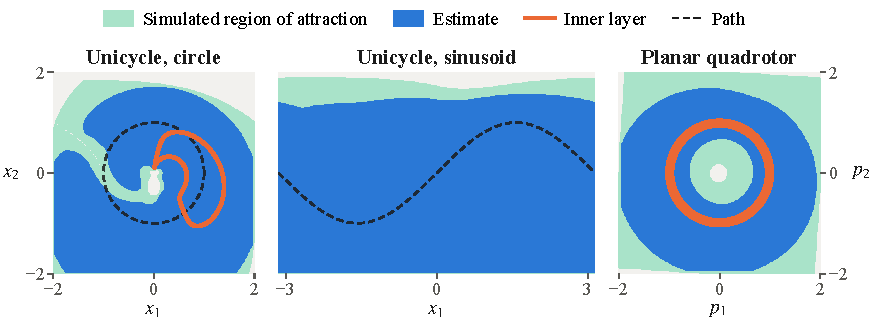
\includegraphics[width=\linewidth]{fig_slices3}

\vspace{-0.1in}

\caption{Slices of the three cases. The unicycle slices are at heading north and speed $1$, and the quadrotor slice is at the orbit velocity,
level tilt and hover thrust. The estimate is the union of the outer layers of four seeds.}
\label{fig:slices}

\vspace{-0.35in}

\end{figure}

\paragraph{How large are the estimates?} The estimates cover most of the simulated region of attraction on the unicycle and a small part of it on the quadrotor
(Table~\ref{tab:main}). The mean single-seed coverage is \resCovCircMean, \resCovSinMean\ and \resCovQuadMean\ on the circle, the sinusoid and the quadrotor, and the unions of four
seeds cover \resAbsCirc, \resAbsSin\ and \resAbsQuad. The inner layer alone covers \resAbsInnerCirc, \resAbsInnerSin\ and \resAbsInnerQuad. Cut at the level of the candidate, the exact
value function covers \resCeilCirc\ and \resCeilSin\ on the unicycle, and the outer layers reach \resCeilFracCirc\ and \resCeilFracSin\ of these shares. Fine-tuning
raises the mean single-seed coverage from \resRawCircMean\ to \resCovCircMean\ on the circle and from \resRawSinMean\ to \resCovSinMean\ on the sinusoid. On the
quadrotor, screening kept the trained network in \resKeptQuad\ of four runs, so its coverage before and after fine-tuning differs only through the draw of the
final test (Appendix~\ref{app:extra}). \resFPSentence\ inside an estimate and outside the simulated region of attraction.
The direct test of unsafe states, with $10^6$ i.i.d.\ box samples per case, finds \resUnsafeKCirc, \resUnsafeKSin\ and
\resUnsafeKQuad\ unsafe samples in the unions of four estimates. With confidence $1-10^{-6}$ and up to the integration error, the states of each union
outside $\D(M)$ therefore occupy at most \resUnsafeEpsCirc, \resUnsafeEpsSin\ and \resUnsafeEpsQuad\ of the box (Appendix~\ref{app:extra}). Each unsafe sample in an estimate shows that the final test missed counterexamples in the annulus of that seed, as
Proposition~\ref{prop:scen} allows.

The quadrotor is the hardest of the three cases. It has
six states, and its inner layer is negligible because thrust enters the error coordinates only through the accelerations, so states near zero thrust
have a small quadratic cost-to-go (Appendix~\ref{app:extra}). On the quadrotor only the candidate and the safety-value baseline, the two
functions built on a learned safety value function, cover more than \resOtherMaxQuad. Counterexamples hold the selected levels of the quadrotor between \resCtwoMinQuad\ and \resCtwoMaxQuad. At these levels the bound
$V_\theta\ge\gamma\qex$ alone excludes \resFloorQuad\ of its simulated region of attraction, and the exact value function covers only \resCeilQuad\
(Table~\ref{tab:main}). The quadrotor estimate can therefore grow only if the level rises (Appendix~\ref{app:extra}).

\paragraph{Does the decomposition matter?} It does on all three cases, and on the quadrotor the safety-value baseline nearly matches the candidate. The candidate covers \resGapCirc, \resGapSin\ and \resGapQuad\ points more than the no-decomposition baseline, which covers \resWholeCirc, \resWholeSin\ and \resWholeQuad\ under the same tests.
This baseline must learn the integral of the running cost, and on the quadrotor counterexamples hold its level below \resWholeLevelMaxQuad. The safety-value baseline has no running cost. On seed 0, before fine-tuning, it covers \resSafetyCirc, \resSafetySin\ and \resSafetyQuad, against \resSeedZeroCirc, \resSeedZeroSin\ and \resSeedZeroQuad\ for the candidate (Table~\ref{tab:ablation}). On the quadrotor this difference is smaller than the change of up to \resDrawMaxQuad\ points that a new draw of the final test causes on a single seed (Appendix~\ref{app:extra}).

\paragraph{How do the PINN baselines compare?} They cover much less than the candidate on all three cases. The Zubov PINN covers \resPinnTFLCirc, \resPinnTFLSin\ and \resPinnTFLQuad, the Dirichlet-Zubov PINN \resDzTFLCirc, \resDzTFLSin\ and \resDzTFLQuad, and the quadratic
baseline \resQuadCirc, \resQuadSin\ and \resQuadQuad. Both PINNs use simulated labels, and the candidate uses none. On the circle and the quadrotor the Zubov PINN takes values
at or near zero at sampled states outside the inner layer. Level selection then returns a level of at most \resPinnLevelMax, and the estimate reduces to the inner layer. The estimate of the Dirichlet-Zubov PINN reduces to the inner layer in the same way on the sinusoid and the quadrotor. Appendix~\ref{app:bench} also trains
both PINNs with the features and the network of the candidate.

\paragraph{Limitations.} The simulated region of attraction comes from a finite-time simulation, and a four-times finer step changes at most \resRefNoiseMax\ of its labels
(Appendix~\ref{app:extra}). The method needs the model, both to integrate steps and to form $\qex$. An uncertain model would require the perturbed value function of
\citet{gruene2015}. The quadrotor is planar with a rate-controlled attitude, and we did not attempt the spatial quadrotor, which has twelve states before dynamic extension.

\begin{table}[t]
\centering\footnotesize\setlength{\tabcolsep}{2.5pt}
\caption{Coverage (\%) on the equilibrium benchmarks, mean $\pm$ std over four seeds where shown. Below the line: the obstacle benchmarks of \citet{mengliu2026}. Zubov PINN: searched scale. n/a: not run. FP as in Table~\ref{tab:main}.}
\label{tab:bench}
\begin{tabular}{@{}lccccccccc@{}}
\toprule
System & \shortstack{Share\\of box} & Quadratic & SOS & \shortstack{Zubov\\PINN} & \shortstack{Dirichlet-\\Zubov PINN} & \shortstack{Ours,\\before} & \shortstack{Ours,\\seed} & \shortstack{Ours,\\union} & FP\\
\midrule
Van der Pol, $\mu=1$ & 39.2 & 77.8 & 99.1 & $98.9\pm0.4$ & $97.2\pm0.5$ & $98.6\pm0.4$ & $98.6\pm0.4$ & 99.2 & 0.00\\
Van der Pol, $\mu=3$ & 28.4 & 55.8 & 93.3 & $91.5\pm3.1$ & $94.8\pm1.6$ & $79.0\pm6.5$ & $90.4\pm2.0$ & 93.8 & 0.00\\
Pendulum, $|u|\le0.8$ & 32.3 & 14.7 & 53.8 & $99.2\pm0.2$ & $91.5\pm1.1$ & $87.5\pm2.0$ & $91.6\pm1.4$ & 93.2 & 0.00\\
3-D, constraint and obstacle & 59.0 & 2.1 & 10.0 & $61.2\pm3.9$ & $70.9\pm1.0$ & $70.6\pm3.2$ & $82.8\pm1.2$ & 85.6 & 0.00\\
Power system & 33.1 & 25.1 & 43.8 & $98.6\pm0.4$ & $90.6\pm1.6$ & $90.8\pm1.2$ & $92.5\pm1.7$ & 96.0 & 0.00\\
\midrule
Van der Pol, 1 obstacle & 33.9 & 21.0 & n/a & $80.9\pm2.1$ & $87.4\pm1.5$ & $78.8\pm5.7$ & $85.5\pm3.0$ & 89.9 & 0.00\\
Van der Pol, 2 obstacles & 28.5 & 24.9 & n/a & $56.1\pm1.1$ & $78.6\pm2.3$ & $59.0\pm6.7$ & $66.5\pm5.5$ & 73.4 & 0.00\\
Power, 2 obstacles & 23.6 & 7.2 & n/a & $73.1\pm0.9$ & $86.4\pm3.1$ & $73.6\pm7.3$ & $74.0\pm6.4$ & 81.0 & 0.00\\
Power, 4 obstacles & 20.3 & 32.9 & n/a & $76.0\pm1.8$ & $90.8\pm1.8$ & $64.5\pm3.2$ & $64.8\pm2.9$ & 75.7 & 0.00\\
\bottomrule
\end{tabular}
\end{table}


\subsection{Equilibrium benchmarks}\label{sec:bench}
\paragraph{Does the learning extend beyond TFL?} It does, and its largest advantages over the PINNs are on the 3-D system and on the power system
with two obstacles. The upper block of Table~\ref{tab:bench} reports five benchmarks: two reversed Van der Pol oscillators, a pendulum with torque saturation,
a 3-D system with a state limit and an obstacle, and a two-machine power system. The lower block adds the four obstacle benchmarks of \citet{mengliu2026}
(Appendix~\ref{app:bench}). We use the construction of Section~\ref{sec:general} with four seeds each, and every method except sum-of-squares is scored with
the verified inner layer $E$. \resBenchFPSentence\ inside an estimate and outside the simulated region of attraction. The candidate is fine-tuned and the PINNs
are not, so the table also gives its coverage before fine-tuning. The candidate covers more than the quadratic baseline on every benchmark, and it covers the
most on \resObsBestCount\ of the five benchmarks with obstacles. Before fine-tuning, it covers the most on \resObsBestBeforeCount\ of them, and the
Dirichlet-Zubov PINN covers more on both oscillators with obstacles. A PINN covers more on \resPinnWinsN\ systems: the Dirichlet-Zubov PINN on the oscillator with
$\mu=3$ and on the power system with four obstacles, and the Zubov PINN on the power system. On the two oscillators, sum-of-squares covers more than the mean
single-seed coverage of the candidate. The direct test of unsafe states finds at most \resAllUnsafeMax\ unsafe samples per system, so $\varepsilon_k$ is at most
\resBUnsafeEpsMax\ in each case. The \resBUnsafePend\ unsafe samples of the pendulum lie in the estimate of \resBUnsafePendSeeds\ seed and converge to a second stable equilibrium of
the saturated loop. Appendix~\ref{app:bench} compares the methods system by system.

% ======================================================================================================
\section{Conclusions}\label{sec:conclusion}
For a TFL controller, the state-constrained Zubov value function of the constrained region of attraction is the sum of a known
quadratic cost-to-go and a safety value function, so only the safety value function has to be learned. The same learning extends to
general closed loops with an equilibrium, where a sublevel set of the quadratic form of the linearization gives the inner layer. In both cases, the estimate has an inner layer
verified by interval branch and bound and an outer layer tested on samples, with confidence bounds on the missed counterexamples and on the
states it wrongly includes. A rigorous flow enclosure on the
annulus would turn the test of the outer layer into a verification, and we leave it to future work. On the quadrotor the estimate stays small,
because counterexamples hold the outer level low and the quadratic lower bound of the value function then excludes \resFloorQuad\ of the simulated region of attraction.
Raising this level is a second direction for future work.

\bibliography{refs3}

\appendix
% Appendices of main.tex
\section{Related Work}\label{app:related}

\paragraph{Zubov functions with constraints.} \citet{camilli2001} extended Zubov's equation to perturbed systems, and
\citet{gruene2015} added state constraints through an obstacle term. Our value function is their equation~(3.4) without the
perturbation. \citet{xue2020} use the same kind of value function with a prescribed running cost built from a polynomial, whose
integral along trajectories is unknown, and compute convex sum-of-squares inner approximations for polynomial systems. Lemma~\ref{lem:split}
gives this integral in closed form for TFL closed loops. Converse Lyapunov-barrier theorems show that a smooth Lyapunov function exists on sets such as $\D(M)$ when the target set is compact and uniformly
asymptotically stable, for perturbed continuous-time systems \citep{meng2022} and for hybrid systems \citep{meng2023}. Such a function is not known in closed form. Neural solvers of Zubov equations \citep{liu2025,liu2024lyznet,kang2023} and their
state-constrained versions in continuous time \citep{mengliu2026} and discrete time \citep{serry2025,serry2026} learn the value function of an
equilibrium or of a compact invariant set. Those that certify the result verify Lie-derivative conditions in continuous time or one-step
conditions in discrete time, with satisfiability-modulo-theories or bound-propagation tools. \citet{xue2020bellman} characterize the interior of the maximal robust region of attraction of an equilibrium of a
state-constrained, perturbed discrete-time system by a Bellman equation, a discrete-time analogue of the equation of \citet{gruene2015}. \citet{serry2026} note that initial estimates of
the region of attraction for non-singleton sets remain open, and our inner layer gives one for TFL closed loops.

\paragraph{Safety value functions and reachability.} Equation~\eqref{eq:dp} is the self-consistency equation of an undiscounted
safety value function \citep{yu2022}, and reach-avoid reinforcement learning uses the same recursion with a frozen target \citep{hsu2021}.
DeepReach solves reachability equations by a residual loss \citep{bansal2021}, and \citet{bokanowski2023} use neural backward recursions for finite-horizon
problems with a maximum running cost and obstacles. The closest precedent for our problem is \citet{oishi2006}, who synthesize, on a grid and in low dimension, parameterized feedback-linearizing
controllers together with the set of states on which they satisfy state and saturation limits. Our setting differs in the
target set, the singular decoupling matrix, the learned function, and the known decrease that the running cost provides. In the language of viability theory, $\D(M)$ is the viability kernel of $\Oad$ under the closed loop.

\paragraph{Local estimates and sampled certificates.} \citet{manchester2011} computes inner estimates of the regions of attraction of hybrid limit cycles from a quadratic form on the linearized transverse dynamics. \citet{faulwasser2016} use a sublevel set of a quadratic in transverse coordinates as the terminal region of
a path-following predictive controller, for a global transverse feedback linearization without a singular decoupling matrix. Finite-step Lyapunov conditions go back to
\citet{aeyels1998} and \citet{geiselhart2014}. \citet{bobiti2018} verify a finite-step decrease on samples with Lipschitz margins and glue the
verified annulus to a local set obtained from linearization and a numerical optimizer, and they set the level below the samples that violate the decrease. Our annulus
has the same shape and is tested on samples only, and our inner layer is verified by interval arithmetic. \citet{liu2025} combine a local quadratic region with a neural sublevel set, with
the inclusion checked by a formal verifier. \citet{li2025} certify an annulus above an inner level, and \citet{score2026} certify an annulus statistically above an independently
certified inner set. The anchored networks of \citet{liu2026anchored} give an inclusion of sublevel sets with a constant that depends on the parameters.
Inclusion~(ii) of Theorem~\ref{thm:main} holds with no such constant. \citet{boffi2020} bound the generalization error of certificates learned from
trajectories, and Proposition~\ref{prop:scen} is the one-dimensional case of \citet{campi2008}. \citet{kenanian2019} show by example that a bound on the measure of
counterexamples to the decrease does not bound the measure of non-converging states. \citet{berkenkamp2016} and \citet{richards2018} close the gap between samples and the continuum with
Lipschitz constants on a grid. In our setting the Lipschitz constant grows as the margins to the singular set shrink, which makes such a grid expensive in four to six
dimensions.

\paragraph{Neural Lyapunov functions and TFL.} Neural Lyapunov functions with counterexample-guided training and exact verification
\citep{chang2019,abate2021,dai2021,wu2023,yang2024} reach systems of six to twelve states. \citet{barreau2024} learn a maximal Lyapunov function
as a quadratic plus a signed residual, optimized jointly on a prescribed compact domain. Our candidate shares this additive form. Its quadratic is
fixed and exact on the admissible set, and its network is nonnegative. We found no prior network composed with an obstacle function by a maximum. The TFL literature \citep{nielsen2006,nielsen2008,akhtar2011,akhtar2015,akhtar2012,allawati2026} proves local exponential
stability of the target set and treats regularity as an assumption. For the quadrotor, Assumption~A1 of \citet{allawati2026} assumes nonzero thrust on a neighbourhood of the
path, and their Remark~2 notes that positive thrust is guaranteed only near the path-following manifold.

\section{The Two Systems}\label{app:systems}

\paragraph{Unicycle.} The dynamically extended unicycle, a simpler model than the car-like robot of \citet{akhtar2015} with the same singularity at zero speed, has state $x=(x_1,x_2,x_3,x_4)$ and
\begin{equation}\label{eq:uni}
\dot x_1=(1+x_4)\cos x_3,\quad \dot x_2=(1+x_4)\sin x_3,\quad \dot x_3=u_2,\quad \dot x_4=u_1,
\end{equation}
so $1+x_4$ is the speed, $u_1$ the acceleration and $u_2$ the turn rate. Both outputs have relative degree two,
$\xi=(\alpha,L_f\alpha)$, $\eta=(\varpi,L_f\varpi)$, $\Tm(x)=(\eta,\xi)$, and
\begin{equation}
D(x)=\begin{bmatrix}L_{g_1}L_f\varpi & L_{g_2}L_f\varpi\\ L_{g_1}L_f\alpha & L_{g_2}L_f\alpha\end{bmatrix},\qquad
\det D(x)=\pm(1+x_4)\det\begin{bmatrix}\nabla\varpi\\ \nabla\alpha\end{bmatrix}.
\end{equation}
The controller is \eqref{eq:tfl} with $\nu_\perp=-\xi_1-2\xi_2$ (double pole at $-1$) and $\nu_\parallel=-(\eta_2-1)$, so the
tangential speed $\eta_2=L_f\varpi$ is driven to $\bar\eta=1$. The error coordinates are $z=(\xi_1,\xi_2,\eta_2-1)$ with
$A=\operatorname{blkdiag}\big(\begin{smallmatrix}0&1\\-1&-2\end{smallmatrix}\big),-1\big)$ and $Q=\operatorname{diag}(1.742,0.249,3.281)$.
The target set $M=\{z=0\}$ is the path traversed with tangential speed $\eta_2=1$. For the unicycle it has two components,
with the heading along the path and positive speed, and with the heading against the path and negative speed, because
$\eta_2$ depends on the velocity and not on the heading. On both components, $|\det D|$ and $|\det J_\Tm|$ are bounded away
from zero and the state is inside the box, as the expressions below show, so $M$ is compact and lies in $\Oad$. The
reference simulation counts convergence to either component.

\emph{Circle.} The path is $\alpha=x_1^2+x_2^2-1$ with $\varpi=\operatorname{atan2}(x_2,x_1)$, so
$\xi_2=2(1+x_4)(x_1\cos x_3+x_2\sin x_3)$, $\eta_2=(1+x_4)(x_1\sin x_3-x_2\cos x_3)/(x_1^2+x_2^2)$,
$\det D=-2(1+x_4)$, $\det J_\Tm=4(1+x_4)$, $\|\nabla\varpi\|^{-1}=\sqrt{x_1^2+x_2^2}$. Box: $|x_1|,|x_2|\le2$,
$x_4\in[-3,1]$ (speed in $[-2,2]$), $x_3\in S^1$.
\emph{Sinusoid.} The path is $\alpha=x_2-\sin x_1$ with $\varpi=x_1$, so $\xi_2=(1+x_4)(\sin x_3-\cos x_1\cos x_3)$,
$\eta_2=(1+x_4)\cos x_3$, $\det D=\det J_\Tm=1+x_4$, $\|\nabla\varpi\|^{-1}=1$. The closed loop is $2\pi$-periodic in $x_1$,
taken in $[-\pi,\pi)$. The box is $|x_2|\le2$, $x_4\in[-3,1]$. On $M$ the speed has magnitude $\sqrt{1+\cos^2x_1}\le\sqrt2$.
The thresholds are $\epsilon_D=\epsilon_\Tm=10^{-2}$ and $\epsilon_\varpi=5\cdot10^{-2}$, so $\Oad$ excludes $|1+x_4|\le0.005$ (circle)
or $\le0.01$ (sinusoid) and, for the circle, the disc of radius $0.05$ around the centre.

\paragraph{Planar quadrotor.} The state is $(p_1,p_2,w_1,w_2,\vartheta,T)$ with
\begin{equation}\label{eq:quad}
\dot p=w,\qquad \dot w=T\begin{bmatrix}-\sin\vartheta\\ \cos\vartheta\end{bmatrix}-\begin{bmatrix}0\\1\end{bmatrix},\qquad
\dot\vartheta=u_2,\qquad \dot T=u_1,
\end{equation}
in units with unit mass, unit gravity and unit path radius. The thrust $T$ is a controller state (the dynamic extension of \citet{akhtar2012}),
and the tilt rate is the second input, as provided by a multirotor autopilot with an inner rate loop. For the loop
$\alpha=p_1^2+p_2^2-1$, $\varpi=\operatorname{atan2}(p_2,p_1)$ both outputs have relative degree three:
$\xi=(\alpha,\ 2p^\top w,\ 2|w|^2+2p^\top\dot w)$,
$\eta_2=(p_1w_2-p_2w_1)/|p|^2$ the angular rate, $\eta_3=L_f^2\varpi$, and
\begin{equation}
D(x)=\begin{bmatrix}n_1/|p|^2 & Tn_2/|p|^2\\ 2n_2 & -2Tn_1\end{bmatrix},\qquad
n_1=p_1\cos\vartheta+p_2\sin\vartheta,\quad n_2=p_2\cos\vartheta-p_1\sin\vartheta,
\end{equation}
so $\det D=-2T$ and $\det J_\Tm=-8T$.
The controller is \eqref{eq:tfl} with $\nu_\perp=-8\xi_1-12\xi_2-6\xi_3$ (triple pole at $-2$) and
$\nu_\parallel=-(\eta_2-\tfrac12)-2\eta_3$ (double pole at $-1$). The error coordinates are
$z=(\xi_1,\xi_2,\xi_3,\eta_2-\tfrac12,\eta_3)$ with $Q=I$, and $M=\{z=0\}$ is the loop traversed counter-clockwise at
angular rate $\tfrac12$. On $M$ the thrust is $T=|\dot w+(0,1)|\in[0.75,1.25]$. The box is $|p_i|\le2$, $|w_i|\le2$, $T\in[0,4]$
(thrust-to-weight ratio up to four), $\vartheta\in S^1$. The thresholds are those of the unicycle, so $\Oad$ excludes $T\le0.005$ and the
disc of radius $0.05$ around the centre. The reference simulation treats a sign change of $T$ between two steps as a
departure through the singular set.

\paragraph{Constants.} Table~\ref{tab:consts} lists the scaling $S_z$ and the cost scale $\gamma$. The scale is
$\gamma=3/p_{90}$, where $p_{90}$ is the 90th percentile of $\zeta^\top P\zeta$ over admissible samples. Both are computed
from the model, without simulating trajectories.
\begin{table}[ht]
\centering\small
\caption{Constants computed before training: the cost scale $\gamma$ of the long-step setting and the diagonal of $S_z^{-1}$.}
\label{tab:consts}
\begin{tabular}{@{}lcl@{}}
\toprule
Case & $\gamma$ & $S_z^{-1}$\\
\midrule
Circle & 0.0444 & 1.550, 1.396, 1.011\\
Sinusoid & 0.0608 & 1.001, 0.625, 1.000\\
Quadrotor & 0.0288 & 1.546, 2.439, 5.953, 0.703, 1.034\\
\bottomrule
\end{tabular}
\end{table}


\section{Proofs}\label{app:proofs}

\paragraph{Proof of Lemma~\ref{lem:split}.} By Assumption~\ref{ass:main}(b), the error coordinates satisfy $\dot z=Az$ on $\Oad$, hence $\dot\zeta=\tilde A\zeta$ and
$\frac{d}{dt}\zeta^\top P\zeta=\zeta^\top(\tilde A^\top P+P\tilde A)\zeta=-\zeta^\top Q\zeta$. Integrating along a trajectory in $\Oad$ gives
$\int_0^t\ell=\gamma\qex(x)-\gamma\qex(y(t))$. Substituting in \eqref{eq:V}, $V(x)=\gamma\qex(x)+\sup_{t\ge0}[h(y(t))-\gamma\qex(y(t))]$ when the
trajectory stays in $\Oad$. In that case $z(y(t))\to0$ and the limit points of the trajectory lie in $M$, so $h(y(t))=0$ eventually and $\qex(y(t))\to0$. The supremum is
therefore nonnegative and equals $\sup_t\relu(h-\gamma\qex)(y(t))$. If the trajectory leaves $\Oad$, both sides are infinite by definition. For \eqref{eq:dp}, split the
supremum over $[0,\tau]$ and $[\tau,\infty)$ and use $y(t;x)=y(t-\tau;y(\tau;x))$. \hfill$\square$

Substituting \eqref{eq:split} in the obstacle equation of Theorem~4.4 of \citet{gruene2015} gives, formally, the
variational inequality $\min\{-L_{f_{\mathrm{cl}}}\Phi-\kappa\rho,\ \Phi-\psi\}=0$ on $\Oad$.

\paragraph{Proof of Theorem~\ref{thm:gz}.} Let $y(t;x)$ stay in $\Oad$. By Assumption~\ref{ass:main}(a), the field is bounded on the compact set $\overline{\Oad}$, so the solution exists for all time. Since $\dot z=Az$, $z(y(t))\to0$.
Every limit point of the bounded trajectory lies in $\overline{\Oad}$ and has $z=0$, so it lies in $M$, and $\dist(y(t),M)\to0$. The converse holds by
definition of $\D(M)$. A forward invariant subset of $\Oad$ consists of states that never leave $\Oad$, which gives the maximality. For
$x\in\D(M)$, the closure of the trajectory is a compact subset of $\Oad$, because its limit points lie in $M\subset\Oad$ by Assumption~\ref{ass:main}(c), so $h$ is bounded along
it. By Lemma~\ref{lem:split}, $\int_0^\infty\ell=\gamma\qex(x)<\infty$, and the extra running cost vanishes once the trajectory has entered its
zero set near $M$, so $V(x)<\infty$. Conversely, $V(x)<\infty$ forces $h(y(t;x))<\infty$ for all $t$, so the trajectory never leaves $\Oad$. \hfill$\square$

\paragraph{Proof of Theorem~\ref{thm:main}.} (i) By Lemma~\ref{lem:split}, $\qex$ decreases along the flow on $\Oad$, so a trajectory from $x\in\I$ keeps $\gamma\qex<c_I$
while it stays in $\Oad$. It cannot reach a regularity constraint, because the first such point would have $\gamma\qex<c_I$ by
continuity, and the hypothesis excludes it. It cannot leave $B$, because leaving through a face requires a point where the field points
outward or is tangent, and the hypothesis gives strict inflow at every point of $\{\gamma\qex<c_I\}$ on the faces. So the trajectory stays in $\I$, and
$\I\subset\D(M)$ by Theorem~\ref{thm:gz}. The points of $M$ have $\qex=0$ and lie in $B^\circ$, so $M\subset\I$.
(ii) The inequality $v<c_1$ means $-\ln(1-v)<c_I$, and $\gamma\qex\le-\ln(1-v)$.
(iii) Let $v(x)<c_2$. While $v\ge c_1$, apply a step of the finite-step decrease condition. Each step stays in $\Oad$, has length at
least one and lowers $v$, so the state remains in $\{v<c_2\}$. Either a step reaches $\{v<c_1\}\subset\I$, which is forward invariant in $\Oad$, or
the steps continue forever. In both cases the orbit of $\bar f$ stays in $\Oad$ for all normalized time. By Assumption~\ref{ass:main}(a), the factor $a$ is bounded on
$\overline{\Oad}$, so physical time also diverges, and $x\in\D(M)$ by Theorem~\ref{thm:gz}. \hfill$\square$

\paragraph{Proof of Proposition~\ref{prop:eq}.} The matrix $P$ is positive definite, so $E$ is a compact ellipsoid. A trajectory from $E\setminus\{0\}$ cannot
leave $E$, because it would have to cross $\{q=c_0\}$, where $L_fq<0$, and the origin is an equilibrium. Since $E\subset\Oad$ is compact and forward invariant and
$L_fq<0$ on $E\setminus\{0\}$, LaSalle's invariance principle \citep{khalil2002} shows that every trajectory from $E$ converges to the origin, so $E\subset\D(\{0\})$. Since $\Phi_\theta\ge0$, we have
$V_\theta\ge\gamma q$, and $v_\theta<c_1$ gives $\gamma q\le V_\theta<\gamma c_0$.

For the last claim, note first that $\Phi_\theta\ge\psi$ gives $V_\theta\ge h$. Each term of $h$ tends to infinity as its distance $d_i$ tends to zero,
and the faces of $B$ are among the constraints. For $c<1$ the set $\{v_\theta\le c\}$ therefore keeps every $d_i$ above a positive constant, so it is a
compact subset of $\Oad$ on which $v_\theta$ is continuous. Let $x_0\in\Oad$ with $v_\theta(x_0)<c_2$. While $q(x_k)\ge c_0$, let $x_{k+1}$ be an end point in $\{q<c_0\}$ if one of the horizons
reaches this set along a trajectory in $\Oad$. Otherwise, let $x_{k+1}$ be the end point with the lowest $v_\theta$ among the horizons that satisfy the
finite-step decrease condition at $x_k$. Suppose the sequence never enters $\{q<c_0\}$. The values
$v_\theta(x_k)$ decrease, so all $x_k$ lie in the compact set $K=\{x\in\Oad:\ q(x)\ge c_0,\ v_\theta(x)\le v_\theta(x_0)\}$. A subsequence converges to some
$x_*\in K$, and $v_\theta(x_k)$ decreases to $c_*=v_\theta(x_*)$. The flow of $\bar f$ depends continuously on the initial state, and $\Oad$ and $\{q<c_0\}$ are open. If a horizon $H$ takes $x_*$ to
$\{q<c_0\}$ along a trajectory in $\Oad$, the same holds for every $x_k$ close enough to $x_*$, and the sequence enters $\{q<c_0\}$, a contradiction. Otherwise
$x_*$ satisfies the finite-step decrease condition with some horizon $H$, so its trajectory stays in $\Oad$ over length $H$ and ends at a value below $c_*-\delta$
for some $\delta>0$. For every $x_k$ close enough to $x_*$, the trajectory over the same horizon therefore also stays in $\Oad$ and ends at a value below
$c_*-\delta/2$. The choice of $x_{k+1}$ then gives $v_\theta(x_{k+1})<c_*$, which contradicts $v_\theta(x_k)\downarrow c_*$. After finitely many steps, each along a trajectory in $\Oad$, the
state thus enters $\{q<c_0\}\subset E$, and it then converges to the origin inside $E$. The fields $\bar f$ and $f$ have the same
orbits, and $a\ge1$, so a step of normalized length $H$ takes physical time at most $H$. Hence $x_0\in\D(\{0\})$. \hfill$\square$

\paragraph{Proof of Proposition~\ref{prop:scen}.} Let $G(t)=\mathbb P(\text{counterexamples in }\{c_1\le v<t\})$, nondecreasing and left-continuous. If $G(\bar c_2)\le\varepsilon$
there is nothing to prove. Otherwise let $t_*=\inf\{t:G(t)>\varepsilon\}$. The set $\mathcal C_*$ of counterexamples in
$\{c_1\le v\le t_*\}$ has measure at least $\varepsilon$, the event $G(c_2)>\varepsilon$ requires $c_2>t_*$ and hence no
sample in $\mathcal C_*$, and that has probability at most $(1-\varepsilon)^N$. This is the one-dimensional case of the scenario
theorem of \citet{campi2008}. \hfill$\square$

\paragraph{Proof of Proposition~\ref{prop:unsafe}.} A state of $\mathcal S\setminus U$ lies in $\Oad$ and reaches $\I$ along a trajectory in $\Oad$. By Theorem~\ref{thm:main}(i),
$\I$ is forward invariant and lies in $\D(M)$, so the state lies in $\D(M)$, and $\mathcal S\setminus\D(M)\subset U$. The count $K$ of samples in $U$ is
binomial with parameters $N$ and $p=\mathbb P(U)$. Since $\varepsilon_k$ increases with $k$, the event $p>\varepsilon_K$ is the event $K\le k_*$, with
$k_*$ the largest $k$ such that $\varepsilon_k<p$, and it is empty if there is no such $k$. The distribution function of the binomial at $k_*$
decreases in its success probability, so $\Pr[K\le k_*]\le\Pr[\mathrm{Bin}(N,\varepsilon_{k_*})\le k_*]=10^{-6}$. This is the one-sided
Clopper-Pearson bound. \hfill$\square$

\section{Equilibrium Benchmarks and Baselines}\label{app:bench}
\paragraph{Systems.} Each system has its equilibrium at the origin. Leaving the box counts as leaving $\Oad$. The reversed Van der Pol oscillator is
$\dot x_1=-x_2$, $\dot x_2=x_1-\mu(1-x_1^2)x_2$, on $[-2.5,2.5]\times[-3.5,3.5]$ for $\mu=1$ and $[-3,3]\times[-6,6]$ for $\mu=3$. The pendulum is
$\dot x_1=x_2$, $\dot x_2=\sin x_1-x_2+u$, with $u=\operatorname{sat}_{0.8}(-4.4142x_1-2.3163x_2)$, the gains of Example~5 of \citet{liu2025} and a torque limit that we add, on $[-\pi,\pi]\times[-4,4]$. The 3-D system is $\dot x_1=-x_1+x_2$,
$\dot x_2=0.1x_1-2x_2-x_1^2-0.1x_1^3$, $\dot x_3=-x_3+x_1x_2$, with $x_3<1$ and $(x_1+1)^2+(x_2-1)^2>0.3^2$, on $[-3,3]^2\times[-2,2]$. The power system is
$\dot x_1=x_2$, $\dot x_2=-0.5x_2-\sin(x_1+\pi/3)+\sin(\pi/3)$, on $[-2,3]\times[-3,3]$. The obstacle benchmarks are Examples 3 and 4 of \citet{mengliu2026}. They
use the oscillator with $\mu=1$ on $[-2.5,2.5]\times[-3.5,3.5]$, with a disc of radius $0.25$ at $(1,1)$ and, in the second case, another at $(-1,-1)$. They use the
power system on $[-1,1.5]\times[-1.5,1]$ with discs of radius $1/8$ at $(0.25,\pm0.25)$, and on $[-2,3]\times[-3,1.5]$ with discs of radius $1/4$ at $(2,-1.5)$,
$(-1,0.5)$, $(-1,-1.5)$ and $(\pi/3,0)$. The last disc covers the saddle of the power system. Each disc with centre $o_i$ and radius $r_i$ enters $\Oad$ as the
constraint $\|x-o_i\|-r_i>0$, which gives the admissible set of their obstacle constraints. The reference simulation integrates $5\times10^4$ states with RK4, step $0.01$ and horizon
$40$ ($60$ for the power system), and a state has converged when the scaled state has norm below $10^{-3}$ for one time unit.

\paragraph{Baselines.} The sum-of-squares baseline is the $V$-$s$ iteration with an expanding interior \citep{jarvis2003,topcu2008,packard2010}, with a polynomial
of degree 6 in two dimensions and 4 in three. It works in the state scaled by the half-widths of the box. The shape function and the initial $V_{\mathrm{sos}}$ are the
quadratic form of the linearization. The multiplier of the expanding set has degree at most 4. The multiplier of the decrease condition has degree 4 on the
polynomial systems and 6 on the pendulum and the power system. One multiplier of degree 2 per constraint keeps $\{V_{\mathrm{sos}}\le1\}$ inside the box and, on the 3-D system,
below the limit and outside the obstacle. The iteration stops after three iterations that raise the level of the expanding set by less than $0.1$ percent. On the
pendulum and the power system, the sine is its Taylor polynomial of degree 5 plus a remainder $\mathrm{rem}(x_1)$ with $|\mathrm{rem}|\le x_1^6/720$. The derivative of $V_{\mathrm{sos}}$ is affine in the remainder.
Imposing the decrease condition at $\mathrm{rem}=\pm x_1^6/720$ therefore covers every admissible remainder, as in \citet{topcu2009} and \citet{chesi2005}. The
saturation of the pendulum enters through an auxiliary variable whose real solutions are exactly the saturated input. Each reported set was solved again with Clarabel to the
status optimal. Its multipliers were then projected onto the positive semidefinite cone. With the coefficient residuals absorbed into the Gram matrices, every
condition passed a floating-point test of positive definiteness. On the pendulum the test needed tighter tolerances and facial reduction, and it accepts residuals of the
decrease condition of about $3\times10^{-16}$, the floating-point resolution of the data. The 3-D set passes the test at the level
\resSosLevelConThree\ of $V_{\mathrm{sos}}$, and the table reports that level. A check of the decrease of $V_{\mathrm{sos}}$ on $4\times10^6$ uniform states found no violation in any set. The runs took
\resSosTimePend\ minutes on the pendulum and \resSosTimePower\ on the power system.

\citet{liu2025} report sum-of-squares volumes of $94.17$ and $70.88$ percent on the two Van der Pol systems, with the interior expanding
algorithm of \citet{packard2010}. On the power system they report $18.53$ percent for a Taylor expansion of the model. They do not define this volume.
We ran our code with the settings of \citet{packard2010}. These are the shape function $x^\top x$, the initial quadratic form computed in the unscaled state,
a multiplier of degree 2 for the expanding set, and 30 iterations without the box. The code then covers \resSosLiuSetVdpOne\ and \resSosLiuSetVdpThree\ of the two
Van der Pol systems. The set for $\mu=3$ fails the Gram test at every level down to $0.9$, so its coverage is not certified. On $\mu=3$ we also changed one of our
settings at a time, against \resSosStudyOurs\ with all of them. The shape function $x^\top x$ gives \resSosStudyShape, the initial form computed in the unscaled state
\resSosStudyInitx, and a multiplier of degree 2 \resSosStudySone. Removing the box gives \resSosStudyNobox, so the box costs the baseline \resSosStudyBoxGap\ points. Our larger
coverage comes from the initial form computed in the scaled state, the shape function and the degree of the multiplier.

The Zubov PINN
follows \citet{liu2025}: two hidden layers of 30 tanh units, $W=\tanh(\sigma V)$, residual $\nabla W\cdot f+\sigma\omega(1-W^2)=0$ with $\omega=\|\tilde x\|^2$, a boundary term at the target, and a data term on $3000$
simulated states, trained for $2\times10^4$ Adam steps on batches of $2048$ from $10^5$ collocation points. On the TFL closed loops the residual is divided by $a(x)$ of Section~\ref{sec:problem}, and the running cost in place of $\|\tilde x\|^2$ is $\omega=\zeta^\top Q\zeta$. On the benchmarks each PINN seed gives one final network, and on the TFL closed loops four snapshots are screened. The inputs on the TFL closed loops are the normalized state with angles as sine and cosine. The sublevel sets of both PINNs are restricted to $\Oad$.

\paragraph{Dirichlet-Zubov PINN.} We follow \citet{mengliu2026}. With $d_{\min}=\min_id_i/\mathrm{median}\,d_i$ and their value $\lambda=0.1$, the same residual is solved with the field $\lambda d_{\min}f$. The function is zero at the target and one on the $2000$ admissible states closest to the boundary of $\Oad$. The data term integrates $\omega/(\lambda d_{\min})$ along the simulated trajectories. For uniformity with the TFL closed loops, collocation and the boundary term act on admissible states. On the TFL closed loops the residual is divided by $\sqrt{1+\|S\lambda d_{\min}f\|^2+(\sigma\omega)^2}$, a positive weight. On their obstacle benchmarks our
reimplementation departs from their settings in three ways. The quantity $d_{\min}$ also counts the faces of the box, the network sees the normalized state, and the
scale comes from the search below in place of their fixed values.

\paragraph{Scale search.} For the Zubov PINN we search $\sigma=\gamma/n$ with $n$ in $\{1,3,10,30,100,300\}$ by coverage on seed 0. For the Dirichlet-Zubov PINN the grid is $\{1,3,10,30,100\}$, and on the Van der Pol oscillator with $\mu=1$ it extends to $300$ and $1000$. On the circle and the quadrotor the Zubov PINN ties at the inner layer at every scale, as does the Dirichlet-Zubov PINN on the sinusoid and the quadrotor, and $n=1$ is reported for these ties. On the sinusoid, the smaller scale $n=1/3$ gives no gain for the Zubov PINN. For the Zubov PINN the benchmark table gives the larger mean of the default $n=1$ and the selected scale, because a selection on one seed is unreliable when that seed reduces to the inner layer. On the TFL closed loops we also trained both PINNs on seed 0 with the features and the network of the candidate, at $n=1$ and $n=10$. The better of the two PINNs then covers \resRichMaxCirc, \resRichMaxSin\ and \resRichMaxQuad\ on the three cases. On the oscillator with two obstacles the Zubov PINN selects $n=300$, the largest value of its grid. Neither PINN is fine-tuned.

\paragraph{Other baselines on the TFL closed loops.} The no-decomposition baseline keeps the features of the candidate and its factor $\tanh(\qex/q_0)$. Its function is
$V_\theta=\max\{h,\Psi_\theta\}$, and the running cost $\ell$ is integrated along the short steps and included in the target. Sum-of-squares and moment
methods \citep{xue2020,korda2013} are not applied to the TFL closed loops, which are rational with trigonometric terms and singular.

\paragraph{Scoring.} \citet{liu2025} report formally verified coverage of $95.6$ and $85.1$ percent on the two Van der Pol systems, measured on their own reference set. We score our reimplementation with the level selection and final test of this paper. On the benchmarks the quadratic baseline, the PINNs and the candidate are scored with the verified inner layer $E$ of Appendix~\ref{app:core}. Counterexamples are sought only outside $E$, and a step
that ends in $\{q<c_0\}$ passes. For the quadratic baseline and the PINNs, $c_1$ lies just below the lowest value of the function outside $E$ over the samples. The PINNs are not clipped at
zero, because clipping creates plateaus on which no step can decrease. Without the rule for steps that end in $\{q<c_0\}$, the estimates of \resRedN\ PINN seeds
reduce to $E$. \resRecN\ of them, on the oscillator with $\mu=3$, the pendulum and the power system, have networks that are lower near $E$ than at the origin. The
rule raises these seeds to between \resRecLo\ and \resRecHi\ percent. On the 3-D system the other \resRestN\ stay within \resRestGap\ points of $E$, because their
lowest values lie at states whose step leaves $\Oad$. The final test of each benchmark run reuses the seed of an earlier final test of the
same run. Its samples did not enter the training, the screening, the fine-tuning or the retest, so Proposition~\ref{prop:scen} still applies to the
candidate. The scale search of the PINNs ranked the scales on seed 0 by coverage after this final test, which lowered no level there by more than \resGridLowerMax.



\paragraph{Results on the five benchmarks.} The mean single-seed coverage of the candidate lies between \resBenchSeedMin\ and \resBenchSeedMax. On the oscillator with $\mu=1$, the Zubov PINN and the Dirichlet-Zubov PINN cover \resPinnVdpOne\ and \resDzVdpOne, against \resSeedVdpOne\ for the candidate. With $\mu=3$, the Dirichlet-Zubov PINN covers more than the candidate, \resDzVdpThree\ against \resSeedVdpThree. On the pendulum the Zubov PINN at the searched scale covers about as much as the candidate, \resPinnPend\ against \resSeedPend. On the power system it covers more, \resPinnPower\ against \resSeedPower. On the 3-D system, the one benchmark of the upper block with constraints inside the box, the candidate covers \resSeedConThree, the Dirichlet-Zubov PINN \resDzConThree, sum-of-squares \resSosConThree\ and the Zubov PINN \resPinnConThree. On the two oscillators, sum-of-squares covers more than the mean single-seed coverage and comes within \resSosGapMax\ points of the union of four seeds. On the pendulum and the power system, sum-of-squares with a bound on the Taylor remainder covers \resSosPend\ and \resSosPower. Sum-of-squares estimates rest on a numerical semidefinite certificate, and the outer layers of the candidate are tested on samples.

\paragraph{What do the verified inner layers add?} They give the quadratic baseline, the PINNs and the candidate one common verified inner layer,
and the direct test of unsafe states uses them as its terminal set. They hold \resCoreRoaMin\ to \resCoreRoaMax\ of the simulated regions of attraction
(Table~\ref{tab:core}). The rule for steps that end in $\{q<c_0\}$ changes no estimate of the candidate. On the five systems of the upper block, the direct test
finds \resBUnsafeList\ unsafe samples in the unions, so $\varepsilon_k$ is at most \resBUnsafeEpsMax\ in each case.
The \resBUnsafePend\ unsafe samples of the pendulum lie in the estimate of \resBUnsafePendSeeds\ seed, near the saddle at $(\arcsin0.8,\,0)$ of the saturated loop. They
converge to the stable equilibrium at $(\pi-\arcsin0.8,\,0)$. On \resBUnsafeCmp\ reference states the test disagrees with the reference simulation \resBUnsafeDisWord.

\paragraph{How does the candidate compare on the obstacle benchmarks of Meng and Liu?} The obstacles of the lower block of Table~\ref{tab:bench}
remove \resObsNoObsMin\ to \resObsNoObsMax\ of the box from the simulated region of attraction. Counting an exit from the box as a failure changes no reference
label, although \citet{mengliu2026} treat the box only as a region of interest. With one obstacle on the oscillator, the candidate covers \resSeedObsVdpOne\ against
\resDzObsVdpOne\ for the Dirichlet-Zubov PINN. With two obstacles the two are close, \resSeedObsVdpTwo\ against \resDzObsVdpTwo. On the power system with two
obstacles near the equilibrium, the candidate covers \resSeedObsPowTwo, and neither PINN exceeds \resPinnObsPowTwo. With four obstacles the Dirichlet-Zubov PINN
covers more, \resDzObsPowFour\ against a mean single-seed coverage of \resSeedObsPowFour\ and \resUnionObsPowFour\ for the union of four. \citet{mengliu2026} report formally verified
levels of their learned function and no areas, so we compare with our reimplementation of their method. The direct test of unsafe states finds \resOUnsafeList\
unsafe samples, so $\varepsilon_k$ is at most \resOUnsafeEpsMax, and each of them runs into an obstacle.

\section{Interval Verification of the Inner Layer}\label{app:inner}
The hypotheses of Theorem~\ref{thm:main}(i) are statements about explicit functions on a box, and we check them by interval branch and bound \citep{moore2009}. The box is
split into cells. A cell is discarded when interval arithmetic shows that $\gamma\qex\ge c_I$ on it or that it contains no violating point. A cell contains
no violating point when all distances $d_i$ to the regularity constraints are positive on it and, if it touches a face, the normal component of the field has the
inward sign. The remaining cells are bisected along their widest normalized side until none is left. The checks run on the closed box with the periodic angle
over $[-\pi,\pi]$. The lower bound of the quadratic form is the larger of its eigendecomposition $\sum_k\lambda_k(e_k^\top\zeta)^2$, with each square bounded
below by zero, and $\lambda_{\min}(P)\sum_i\zeta_i^2$. The distances $d_i$ and the field components are the symbolic expressions of Appendix~\ref{app:systems},
evaluated in float64 interval arithmetic with outward rounding by two units in the last place per operation and with enclosed constants. For each case the level
is found by bisection over twelve rounds between zero and the sampled minimum of $\gamma\qex$ over samples outside $\Oad$ and samples on box faces where the field
points outward. The last verified level is multiplied by $0.99$. This one percent reduction absorbs the float32 evaluation of $\qex$ in the training pipeline and
the residual effects of the eigendecomposition of $P$ and the float32 storage of $P$ and $S_z$. Table~\ref{tab:inner} lists the
verified levels, the share of the box in $\I$, the number of cells and the time.
\begin{table}[ht]
\centering\small
\caption{Verified inner layers of the TFL cases, with the cells and time of the final verification.}
\label{tab:inner}
\begin{tabular}{lccccc}
\toprule
Case & $c_I$ & $c_1$ & $\I$ (\% box) & Cells & Time (s)\\
\midrule
Circle & 0.1050 & 0.0997 & 5.40 & 944395 & 588\\
Sinusoid & 0.0509 & 0.0497 & 1.01 & 1047557 & 110\\
Quadrotor & 0.0006 & 0.0006 & 0.00 & 21270981 & 3626\\
\bottomrule
\end{tabular}
\end{table}


\section{Interval Verification of the Inner Layer of an Equilibrium}\label{app:core}
For an equilibrium, the inner layer is $E=\{q\le c_0\}$ with $q(x)=x^\top\hat Px$ and $\hat P=SPS$, where $S$ is the diagonal matrix of inverse half-widths of $B$.
The matrices $S$ and $P$ are the float32 values that the networks use. They are stored with the verification and checked against the pipeline before each run.
They are exact in rational arithmetic, so $\hat P$ is exact, and Sylvester's criterion in exact rationals shows that $\hat P$ is positive definite. The ellipsoid
$E$ has the bounding box $|x_i|\le\sqrt{c_0(\hat P^{-1})_{ii}}$, so its inclusion in the open box is an exact rational test.

The decrease of $q$ vanishes at the origin, so cells near the origin need a separate argument. On a box $B_0$ around the origin on which $f$ is continuously
differentiable, $f(x)=\bar J(x)x$ with $\bar J(x)=\int_0^1Df(tx)\,dt$. Since $B_0$ is convex and contains the origin, $\bar J(x)$ lies in the interval enclosure
$[Df](B_0)$, and $L_fq=x^\top(\hat P\bar J+\bar J^\top\hat P)x$. Let $\Sigma$ be the midpoint and $\Delta$ the entrywise radius of the symmetric interval matrix
$\hat P[Df](B_0)+[Df](B_0)^\top\hat P$. Every symmetric matrix in it has largest eigenvalue at most $\lambda_{\max}(\Sigma)+\|\Delta\|_F$. It therefore suffices that
$-\Sigma-\bar\delta I$ is positive definite for a rational upper bound $\bar\delta\ge\|\Delta\|_F$, which Sylvester's criterion checks in exact rationals, and then $L_fq<0$ on $B_0\setminus\{0\}$.

Branch and bound covers the rest of the bounding box. A cell is discarded when $q>c_0$ on it, or when every constraint other than the faces of $B$ is positive
on it and either $L_fq<0$ on it or it lies in $B_0$. The bound on $L_fq$ is the natural interval extension of $2(\hat Px)\cdot f(x)$, intersected with the
mean-value form where $f$ is smooth on the cell. On the pendulum this requires the saturation to be strictly active or strictly inactive on the whole cell. A cell
below a minimum width, or a cell whose midpoint violates a condition, ends the verification as a failure. The arithmetic is that of Appendix~\ref{app:inner}, with
sine and cosine widened by a further $10^{-15}$. Decimal constants are enclosed by the neighbouring floats unless they are exact, and $\pi$ is enclosed. The constant
$0.1$ of the 3-D system and $\pi/3$ of the power system are enclosed at their exact values. The verification thus concerns the exact field, which the code
evaluates in float32. The largest passing level is found by bisection over twelve rounds below the lowest sampled failure. It is reduced by one percent to absorb the
float32 evaluation of $q$ in the pipeline, and verified again at the reduced level. Table~\ref{tab:core} lists the inner layers. They hold \resCoreRoaMin\ to
\resCoreRoaMax\ of the simulated regions of attraction. The decrease of $q$ limits the level on the two Van der Pol systems and the power system. The obstacle limits it
on the 3-D system, and the minimum cell width on the pendulum.
\begin{table}[ht]
\centering\small
\caption{Verified inner layers $E=\{q\le c_0\}$ of the equilibrium benchmarks. ROA: simulated region of attraction.}
\label{tab:core}
\begin{tabular}{lccccc}
\toprule
System & $c_0$ & $E$ (\% box) & $E$ (\% ROA) & Cells & Time (s)\\
\midrule
Van der Pol, $\mu=1$ & 0.2553 & 17.14 & 43.7 & 827 & 7\\
Van der Pol, $\mu=3$ & 0.06961 & 8.40 & 29.5 & 1335 & 6\\
Pendulum, $|u|\le0.8$ & 0.005401 & 1.01 & 3.1 & 991 & 8\\
3-D, limit and obstacle & 0.0329 & 1.17 & 2.0 & 3289 & 12\\
Power system & 0.1585 & 5.20 & 15.7 & 725 & 7\\
Van der Pol, 1 obstacle & 0.1049 & 7.05 & 20.8 & 453 & 6\\
Van der Pol, 2 obstacles & 0.1049 & 7.05 & 24.7 & 611 & 5\\
Power, 2 obstacles & 0.0483 & 1.70 & 7.1 & 377 & 6\\
Power, 4 obstacles & 0.1689 & 6.09 & 30.0 & 687 & 6\\
\bottomrule
\end{tabular}
\end{table}


\section{Configuration}\label{app:config}
\paragraph{Training setup.} The candidate uses the network, optimizer and collocation points of Table~\ref{tab:config}, with the level selection and
fine-tuning of Section~\ref{sec:method}. The quadrotor uses a weight of $10$ in place of $100$ for the finite-step penalty and no exponential loss weight during
training.

\paragraph{Extra running cost.} With $c_I$ the level of the inner layer, $\rho$ vanishes below $\gamma\qex=c_I/2$ and equals one above $c_I$. The
constant $\kappa$ is $0.3$ when the inner layer holds at least one percent of the box and $0$ otherwise.

\paragraph{Penalties.} The finite-step penalty acts on steps of unit length in $\Oad$ from $x$ to $x_1$. It asks for
$V_\theta(x_1)\le V_\theta(x)-\chi[\gamma(\qex(x)-\qex(x_1))+C_1]$ with $\chi=0.2$ and $C_1$ the quantity $C_s$ of Section~\ref{sec:method} over the unit step,
and it is applied to the values $e^{-V_\theta}$. An error $\delta V$ at level $V$ moves $v$ by only $e^{-V}\delta V$, so without the exponential loss weight the
loss would carry almost no gradient at the levels near one. Every
five epochs, the $10^4$ states of a fresh pool of $2.5\times10^5$ that violate the finite-step penalty most join the data with
four Gaussian neighbours each, in a rolling buffer of $10^5$. The network starts close to $\Phi_\theta=\psi$, which lies below the exact
solution. Table~\ref{tab:config} gives every constant.

\paragraph{Screening and retest.} Screening uses $3\times5\cdot10^4$ box samples and the additional samples of Table~\ref{tab:config}. The three best
snapshots are retested on $5\times10^5$ fresh box samples, and the best one is kept with the lowest level it received.

\begin{table}[H]
\centering\small
\caption{Configuration of every case. Step lengths are in normalized time, except in the reference simulation.}
\label{tab:config}
\begin{tabular}{@{}p{0.17\linewidth}p{0.80\linewidth}@{}}
\toprule
Value function & $b_i=0.1\cdot$median $d_i$, $h=\sum_i\relu(b_i/d_i-1)^2$, $\gamma=3/(\text{90th percentile of }\zeta^\top P\zeta)$\\
Shaping cost & $\kappa=0.3$ if the inner layer holds at least $1\,\%$ of $2\cdot10^5$ box samples, and $\kappa=0$ otherwise. The function $\rho$ is a smooth step from $\gamma\qex=c_I/2$ to $c_I$. The share on the sinusoid is $1.01\,\%$, close to this threshold\\
Network & $\mathcal N_\theta$: 64-64-64 tanh. Features: normalized state (angles as sine and cosine), $\tanh(\zeta/3)$, $\tanh(\tfrac12\ln(d_i/\mathrm{median}\,d_i))$ for the constraints on $\det D$ and $\|\nabla\varpi\|^{-1}$. Softplus sharpness $\beta=10$. The constant $q_0$ is the first percentile of $\qex$ on $2\cdot10^5$ collocation points\\
Collocation & $4\cdot10^5$ Sobol box samples, $10^5$ near the faces, $10^5$ next to the singular set (admissible ones kept)\\
Initialization & The network starts close to $\Phi_\theta=\psi$, which lies below the exact solution\\
Fitted value iteration & $\tau=0.2$, 8 RK4 substeps. Target network: copy of the averaged weights (decay $0.999$), refreshed every epoch\\
Optimization & Adam, 100 epochs, batch 4096, cosine learning rate $10^{-3}\to10^{-5}$. Exponential loss weight $e^{2\min(V_\theta,V_{\max})}$ with $V_{\max}=3$ (no such weight on the quadrotor).\\
Decrease penalty & Weight 10, on $\relu((L_{f_{\mathrm{cl}}}\Phi_\theta+\kappa\rho)/a)\,e^{-V_\theta}$, where $\Psi_\theta>\psi$\\
Obstacle penalty & Weight 10, on $\relu(\psi+0.01-\Psi_\theta)\,e^{-V_\theta}$, where $\Psi_\theta\le\psi$ and $L_{f_{\mathrm{cl}}}\psi+\kappa\rho>0$\\
Finite-step penalty & Weight 100 (10 on the quadrotor), unit step with 40 RK4 substeps, on $\relu(e^{-(V_\theta(x)-\chi\Delta)}-e^{-V_\theta(x_1)})$ with $\Delta=\gamma\relu(\qex(x)-\qex(x_1))+C_1$ and $\chi=0.2$, on steps in $\Oad$ with $V_\theta(x)<8$.\\
Violating states & Every 5 epochs up to epoch 90: the $10^4$ states whose unit step violates the decrease most (no margin), in a pool of $2\cdot10^5$ box samples and $5\cdot10^4$ next to the singular set, 4 Gaussian neighbours (standard deviation $0.01$ of the half-widths), rolling buffer $10^5$\\
Level selection & Horizons $H\in\{1,2,4,8\}$, RK4 substep $0.025$, states with $\|\zeta\|\le10^{-3}$, which lie in $\I$, exempt from the decrease. Snapshots every 5 epochs and at epoch 0. A test on $n$ box samples adds $n/2$ near the faces, $n/5$ next to the singular set and $n/2$ on the faces, where states with outward field count as counterexamples. Screening $n=5\cdot10^4$, 3 rounds. Retest of the top 3, $n=10^5$, 5 rounds. Ranking by share of $5\cdot10^4$ fixed box samples. Final test: $10^6$ i.i.d.\ uniform box samples\\
Fine-tuning & 4 rounds, pool of $10^6$ box samples, $5\cdot10^5$ near the faces and $2\cdot10^5$ next to the singular set, 8 Gaussian neighbours per counterexample, 300 Adam steps (learning rate $5\cdot10^{-5}$, batch 4096), weight 100 on counterexamples whose step stays in $\Oad$, weight 10 on those that leave it, decrease margin 0.2, counterexample sets capped at $5\cdot10^4$, anchor on $2\cdot10^5$ box samples, exponential loss weight with $V_{\max}=3$ on all systems\\
Reference & $5\cdot10^4$ Sobol states, RK4 step 0.01, horizon 30 (unicycle) and 40 (quadrotor). Converged: held for one time unit, $\|\xi\|<10^{-3}$ and $|\eta_2-1|<0.05$ (unicycle), $\|\zeta\|<10^{-3}$ (quadrotor). States that have neither converged nor failed at the horizon count as outside\\
\bottomrule
\end{tabular}
\end{table}


\section{Additional Results}\label{app:extra}
\paragraph{Unsafe samples and the final test.} The direct test of unsafe states draws $10^6$ i.i.d.\ box samples per case and simulates each sample in the union of the four
estimates until it reaches the inner layer. Of the \resUnsafeInCirc, \resUnsafeInSin\ and \resUnsafeInQuad\ samples in the unions,
\resUnsafeKCirc, \resUnsafeKSin\ and \resUnsafeKQuad\ leave the box first, and finer integration confirms all \resUnsafeConfirmed.
These counts give the bounds of Section~\ref{sec:exp}, and each bound holds for every seed. By Theorem~\ref{thm:main}(iii), the annulus of every
seed whose estimate contains an unsafe sample holds counterexamples that the final test missed. The final test found a counterexample and lowered the level in \resIidFailures\ of
the twelve runs (Table~\ref{tab:seeds}).

\paragraph{How reliable is the direct test of unsafe states?} It is at least as accurate as the reference simulation. The test uses seeds
disjoint from all other tests, the RK4 integration of the normalized field with substeps of length $0.025$ as in the final test, and $t_{\max}=200$. Every sample that reached $\I$ did so within \resUnsafeTimeMax\ units of normalized time. On \resUnsafeCmp\ reference states, the test
and the reference simulation disagree on \resUnsafeDis, and the reference simulation with a four times finer step agrees with the test on
\resUnsafeAgree\ of them. In the other \resUnsafeCons, the test counts as unsafe a state that the finer reference finds converging, which is
the conservative direction. None of the disagreeing states lies in an estimate, so this comparison does not test the safe labels inside the
estimates. The \resUnsafeTotal\ samples counted as unsafe still leave $\Oad$ with four and sixteen times finer substeps, and the reference
simulation with step $0.001$ finds that they leave the box.

\paragraph{What do the two tests leave open?} With $N=10^6$ and $\varepsilon=\ln(10^6)/N=1.38\times10^{-5}$, Proposition~\ref{prop:scen} says
with confidence $1-10^{-6}$ that the uniform measure of counterexamples in the annulus is at most $\varepsilon$. This alone does not bound the measure
of states of the outer layer outside $\D(M)$, because a function can decrease everywhere except on a set of small measure while
most trajectories diverge \citep{kenanian2019}. Both tests integrate numerically and check
membership in $\Oad$ at substeps of length $0.025$, so a crossing of the singular set between substeps could go unnoticed. The test of
Proposition~\ref{prop:unsafe} also checks the sign of $\det D$ at every substep, which rules this out for the zero set of $\det D$ but not for
the other constraints. The union of the outer layers over several seeds is therefore also tested on
samples only. A deterministic check of the hypothesis of Theorem~\ref{thm:main}(iii) needs an enclosure of the flow over a unit step on every cell of the annulus, and we did not
compute one.

\paragraph{What limits the outer layer?} The level limits it on the unicycle, and both the level and the fit limit it on the quadrotor. The exact value function cut at the
level of the candidate covers \resCeilCirc, \resCeilSin\ and \resCeilQuad\ of the simulated region of attraction. The outer layers cover \resCeilFracCirc, \resCeilFracSin\
and \resCeilFracQuad\ of these shares. On the unicycle the levels lie above \resCtwoMinSin, and most of the uncovered states have an exact value function $v$ above $c_2$. Their trajectories pass
near a constraint before converging, so they have a large $\Phi$, and only a level closer to one would include them. On the quadrotor, counterexamples hold the level between
\resCtwoMinQuad\ and \resCtwoMaxQuad, while the exact value function cut at $0.9$ covers \resCeilNineQuad. At these levels the bound $V_\theta\ge\gamma\qex$ excludes \resFloorQuad\ of the simulated region of attraction, against \resFloorCirc\ on the circle and
\resFloorSin\ on the sinusoid.

\paragraph{What do the components contribute?} Fine-tuning helps on the unicycle and changes nothing on the quadrotor. On the quadrotor, screening kept the trained network in
\resKeptQuad\ of four runs. The quadrotor entries before and after fine-tuning in Table~\ref{tab:seeds} therefore differ only through the draw of the final test. This draw alone moves
the coverage of a seed by up to \resDrawMaxQuad\ points. Table~\ref{tab:ablation} removes components on the circle, where the PDE residual loss in place of fitted value iteration reaches \resPinnCirc.

\paragraph{Does the integration step change the reference labels?} It changes few of them. We simulated $5000$ of the $5\times10^4$ reference states of each case again with an RK4 step of $0.0025$ in place of $0.01$. The label changes on \resRefNoiseCirc, \resRefNoiseSin\ and \resRefNoiseQuad\ of these states on the circle, the sinusoid and the quadrotor.

\paragraph{What limits the inner layer?} Contact with the constraints bounds it from above, and the interval verification stops below that bound. On samples, the sublevel sets of $\gamma\qex$
first meet a regularity constraint or a face of the box where the field points outward at levels of at most \resContactCirc, \resContactSin\ and \resContactQuad\ on the three cases. The verified levels are \resCICirc, \resCISin\ and
\resCIQuad\ (Table~\ref{tab:inner}), and on the quadrotor the verification at the next level exceeds its budget of cells. The first contact lies near the centre of the circle, on the speed limit for the sinusoid, and on the
zero-thrust face for the quadrotor. Thrust enters $z$ only through the acceleration coordinates, so a state with no thrust can have a small $\qex$, and the inner layer of the
quadrotor is negligible.

\paragraph{Computation time.} All computations run on the CPU of a laptop (Apple M1). With three cases running at once, training takes \resTimeTrain\ per seed,
level selection \resTimeCert, fine-tuning \resTimeRepair, and the interval verification \resTimeInner.

\begin{table}[ht]
\centering\footnotesize\setlength{\tabcolsep}{3pt}
\caption{Per-seed results. Before: the trained network. Round: selected fine-tuning round (0 is the trained network). Sel.\ and Final: level after the retest and after the final test. Annulus: final-test samples between $c_1$ and the selected level. FP as in Table~\ref{tab:main}.}
\label{tab:seeds}
\begin{tabular}{llcccccccc}
\toprule
Case & Seed & $c_2$ before & Cov.\ before & Round & $c_2$ sel. & $c_2$ final & Annulus & Cov. & FP\\
\midrule
Circle & 0 & 0.9335 & 69.84 & 4 & 0.9835 & 0.9835 & 574093 & 73.82 & 0.000\\
Circle & 1 & 0.9328 & 69.98 & 4 & 0.9855 & 0.9822 & 587824 & 73.31 & 0.000\\
Circle & 2 & 0.9347 & 69.52 & 4 & 0.9877 & 0.9877 & 586506 & 74.81 & 0.000\\
Circle & 3 & 0.9384 & 68.73 & 4 & 0.9869 & 0.9866 & 586012 & 74.01 & 0.000\\
Sinusoid & 0 & 0.8583 & 57.16 & 3 & 0.9784 & 0.9784 & 682245 & 72.77 & 0.000\\
Sinusoid & 1 & 0.8980 & 62.53 & 2 & 0.9808 & 0.9670 & 698328 & 70.32 & 0.000\\
Sinusoid & 2 & 0.8871 & 58.11 & 2 & 0.9749 & 0.9749 & 659706 & 70.39 & 0.000\\
Sinusoid & 3 & 0.8359 & 54.29 & 2 & 0.9607 & 0.9607 & 640343 & 68.29 & 0.000\\
Quadrotor & 0 & 0.3240 & 9.39 & 0 & 0.4337 & 0.3835 & 75400 & 11.57 & 0.000\\
Quadrotor & 1 & 0.3099 & 7.95 & 0 & 0.4327 & 0.2795 & 69250 & 6.83 & 0.000\\
Quadrotor & 2 & 0.3647 & 10.02 & 0 & 0.3800 & 0.3119 & 59678 & 8.12 & 0.000\\
Quadrotor & 3 & 0.4471 & 10.10 & 0 & 0.4471 & 0.4471 & 56764 & 10.10 & 0.000\\
\bottomrule
\end{tabular}
\end{table}

\begin{table}[ht]
\centering\small
\caption{Ablations on seed 0 before fine-tuning, with the same level selection and final test. FP as in Table~\ref{tab:main}.}
\label{tab:ablation}
\begin{tabular}{llccc}
\toprule
Case & Variant & $c_2$ & Coverage & FP\\
\midrule
Circle & full method & 0.933 & 69.8 & 0.00\\
Circle & PDE residual loss in place of fitted value iteration & 0.256 & 9.4 & 0.00\\
Circle & safety-value baseline & 0.781 & 33.5 & 0.00\\
Circle & no finite-step penalty, no counterexamples & 0.629 & 38.8 & 0.00\\
Circle & no exponential loss weight & 0.910 & 64.2 & 0.00\\
Circle & sum form $\Phi=\psi+\Psi_\theta$ & 0.974 & 33.4 & 0.00\\
Sinusoid & full method & 0.858 & 57.2 & 0.00\\
Sinusoid & safety-value baseline & 0.860 & 29.5 & 0.00\\
Quadrotor & full method & 0.324 & 9.4 & 0.00\\
Quadrotor & safety-value baseline & 0.609 & 8.4 & 0.00\\
\bottomrule
\end{tabular}
\end{table}



\end{document}
